\documentclass{article}
\usepackage{ITB_MSCe}
\usepackage{tcolorbox}
\tcbuselibrary{breakable}
\usepackage{bold-extra} % bold tt
\usepackage{lipsum}
\usepackage{graphicx}
\usepackage{color}
\usepackage{amsthm}
\usepackage{amssymb}
\usepackage{amsmath}
\usepackage{amsfonts}
\usepackage{amstext}
\usepackage{latexsym}
\usepackage{upgreek}
\usepackage{hyperref}
\usepackage{url}
\usepackage{nicefrac}
\usepackage{pifont}
\usepackage{marvosym}
\usepackage{enumitem}
\usepackage{tikz}
\usepackage[numbers]{natbib}
\usepackage{eso-pic}
\usepackage{textcomp}
\usepackage{fancyvrb}
\usepackage{mwe}
\usepackage{lastpage}
\usepackage{listings, xcolor}
\usepackage{algorithmic}
\usepackage{algorithm}

\usepackage{array}
\usepackage{ragged2e}
%\bibpunct{}{}{;}{a}{,}{,}

\input{images/rgb}

\lstdefinestyle{python_code}{%
  language=Python, basicstyle=\ttfamily, columns=fullflexible,
  keywordstyle=\color{blue}, commentstyle=\itshape\color{green!50!black},
  stringstyle=\color{magenta}, showstringspaces=false,
  morekeywords={as,@staticmethod}, }

\lstset{ style=python_code }

\newsavebox{\sclbox}

\newcolumntype{L}[1]{>{\RaggedRight}p{#1}}



\newenvironment{declaration}
  {\noindent\textbf{Declaration:}} {\par}

\title{Explaining the policy--practice gap in AI education governance using
multi-layered NLP: A comparative study}

\author{
\normalsize
\begin{tabular}[t]{c@{\extracolsep{1em}}c} Mariem NSIRI & Geraldine GRAY\\
Technological University Dublin & Technological University Dublin\\
B00177462@myTUDublin.ie & supervisor.name@tudublin.ie
\end{tabular}
}

%\date{\today}


\begin{document}

\section{Topic Modelling}

\subsection{Latent Dirichlet Allocation as a first baseline}

LDA was used as the first topic-discovery baseline for
both the policy corpus and the sentiment corpus. LDA represents each document as a
mixture of latent topics and each topic as a probability distribution over words
\cite{blei2003latent}. This makes it a useful first-shot model before moving to
embedding-based or factorisation-based methods: it provides a transparent
bag-of-words reference point and makes it possible to check whether the major themes
of the corpus can already be recovered from lexical evidence alone.

The goal of this LDA stage was exploratory. It was not used as the final topic
interpretation layer. Instead, it was used to create an initial map of the policy and
sentiment corpora, to inspect the behaviour of topic-number selection, and to test
whether synthetic sentiment chunks can distort the discovered topic structure. This
is consistent with the role of topic models in policy-text analysis, where the model
is used to support interpretation rather than replace human review
\cite{isoaho2021topic,chang2009reading}. The implementation is available in the
project repository under this link\footnote{\href{https://github.com/nsirimai/mscdsa/blob/main/msc/progress/topic_modelling/lda/policy/lda_topic_modelling.ipynb}{\texttt{github.com/nsirimai/mscdsa/blob/main/msc/progress/topic\_modelling/lda/policy/lda\_topic\_modelling.ipynb}}}

\subsection{Policy LDA pipeline}

The policy LDA pipeline follows the same preparation logic as the earlier corpus
construction stage. Policy chunks were first checked for metadata consistency, then
cleaned to remove boilerplate, references, contents-page artefacts, very weak chunks
and duplicates. The remaining chunks were lowercased, tokenised, lemmatised and
converted into a dictionary and document--term matrix. Candidate LDA models were then
trained over a range of topic numbers, and the final model was selected using a
combination of topic coherence and topic diversity.

\begin{verbatim}
Policy documents
  -> chunk selection and metadata check
  -> boilerplate, reference and contents-page cleanup
  -> lowercase, tokenise, remove stopwords, lemmatise
  -> remove weak, short or duplicate chunks
  -> build dictionary and document-term matrix
  -> search LDA topic numbers using coherence and diversity
  -> fit global policy model and per-country models
\end{verbatim}

The policy LDA pipeline loaded 1,843 chunks and retained 1,724 chunks for global LDA.
The retained global corpus contained 496 chunks from the USA, 403 from Ireland, 319
from Australia, 308 from France and 198 from UNESCO. The global LDA search selected
four topics, with coherence equal to 0.7021 and diversity equal to 0.9000 (see
Figure~\ref{fig:lda-policy-global-search}). The main global signals were privacy,
bias, risk, guidance, teaching, assessment, skills, ethics, children, literacy,
regulation, digital tools and education policy.

Coherence was used because it evaluates whether the top words of a topic form an
interpretable semantic group. Topic coherence has been proposed as a more
human-facing alternative to likelihood-only evaluation, and different coherence
measures have been shown to correlate better with human judgements of topic
quality~\cite{newman2010automatic,roder2015exploring}. Topic diversity was used as a
complementary metric to penalise repeated topics; coherent topics are not sufficient
if several topics reuse the same terms and therefore fail to separate the corpus into
distinct themes~\cite{dieng2020topic}. The number of topics was therefore treated as
a model-selection problem rather than a cosmetic display choice, following earlier
work on estimating the natural number of LDA topics
\cite{arun2010finding,cao2009density}. This made LDA a controlled baseline before
moving to more flexible topic-modelling pipelines.

\begin{figure}[t]
    \centering
    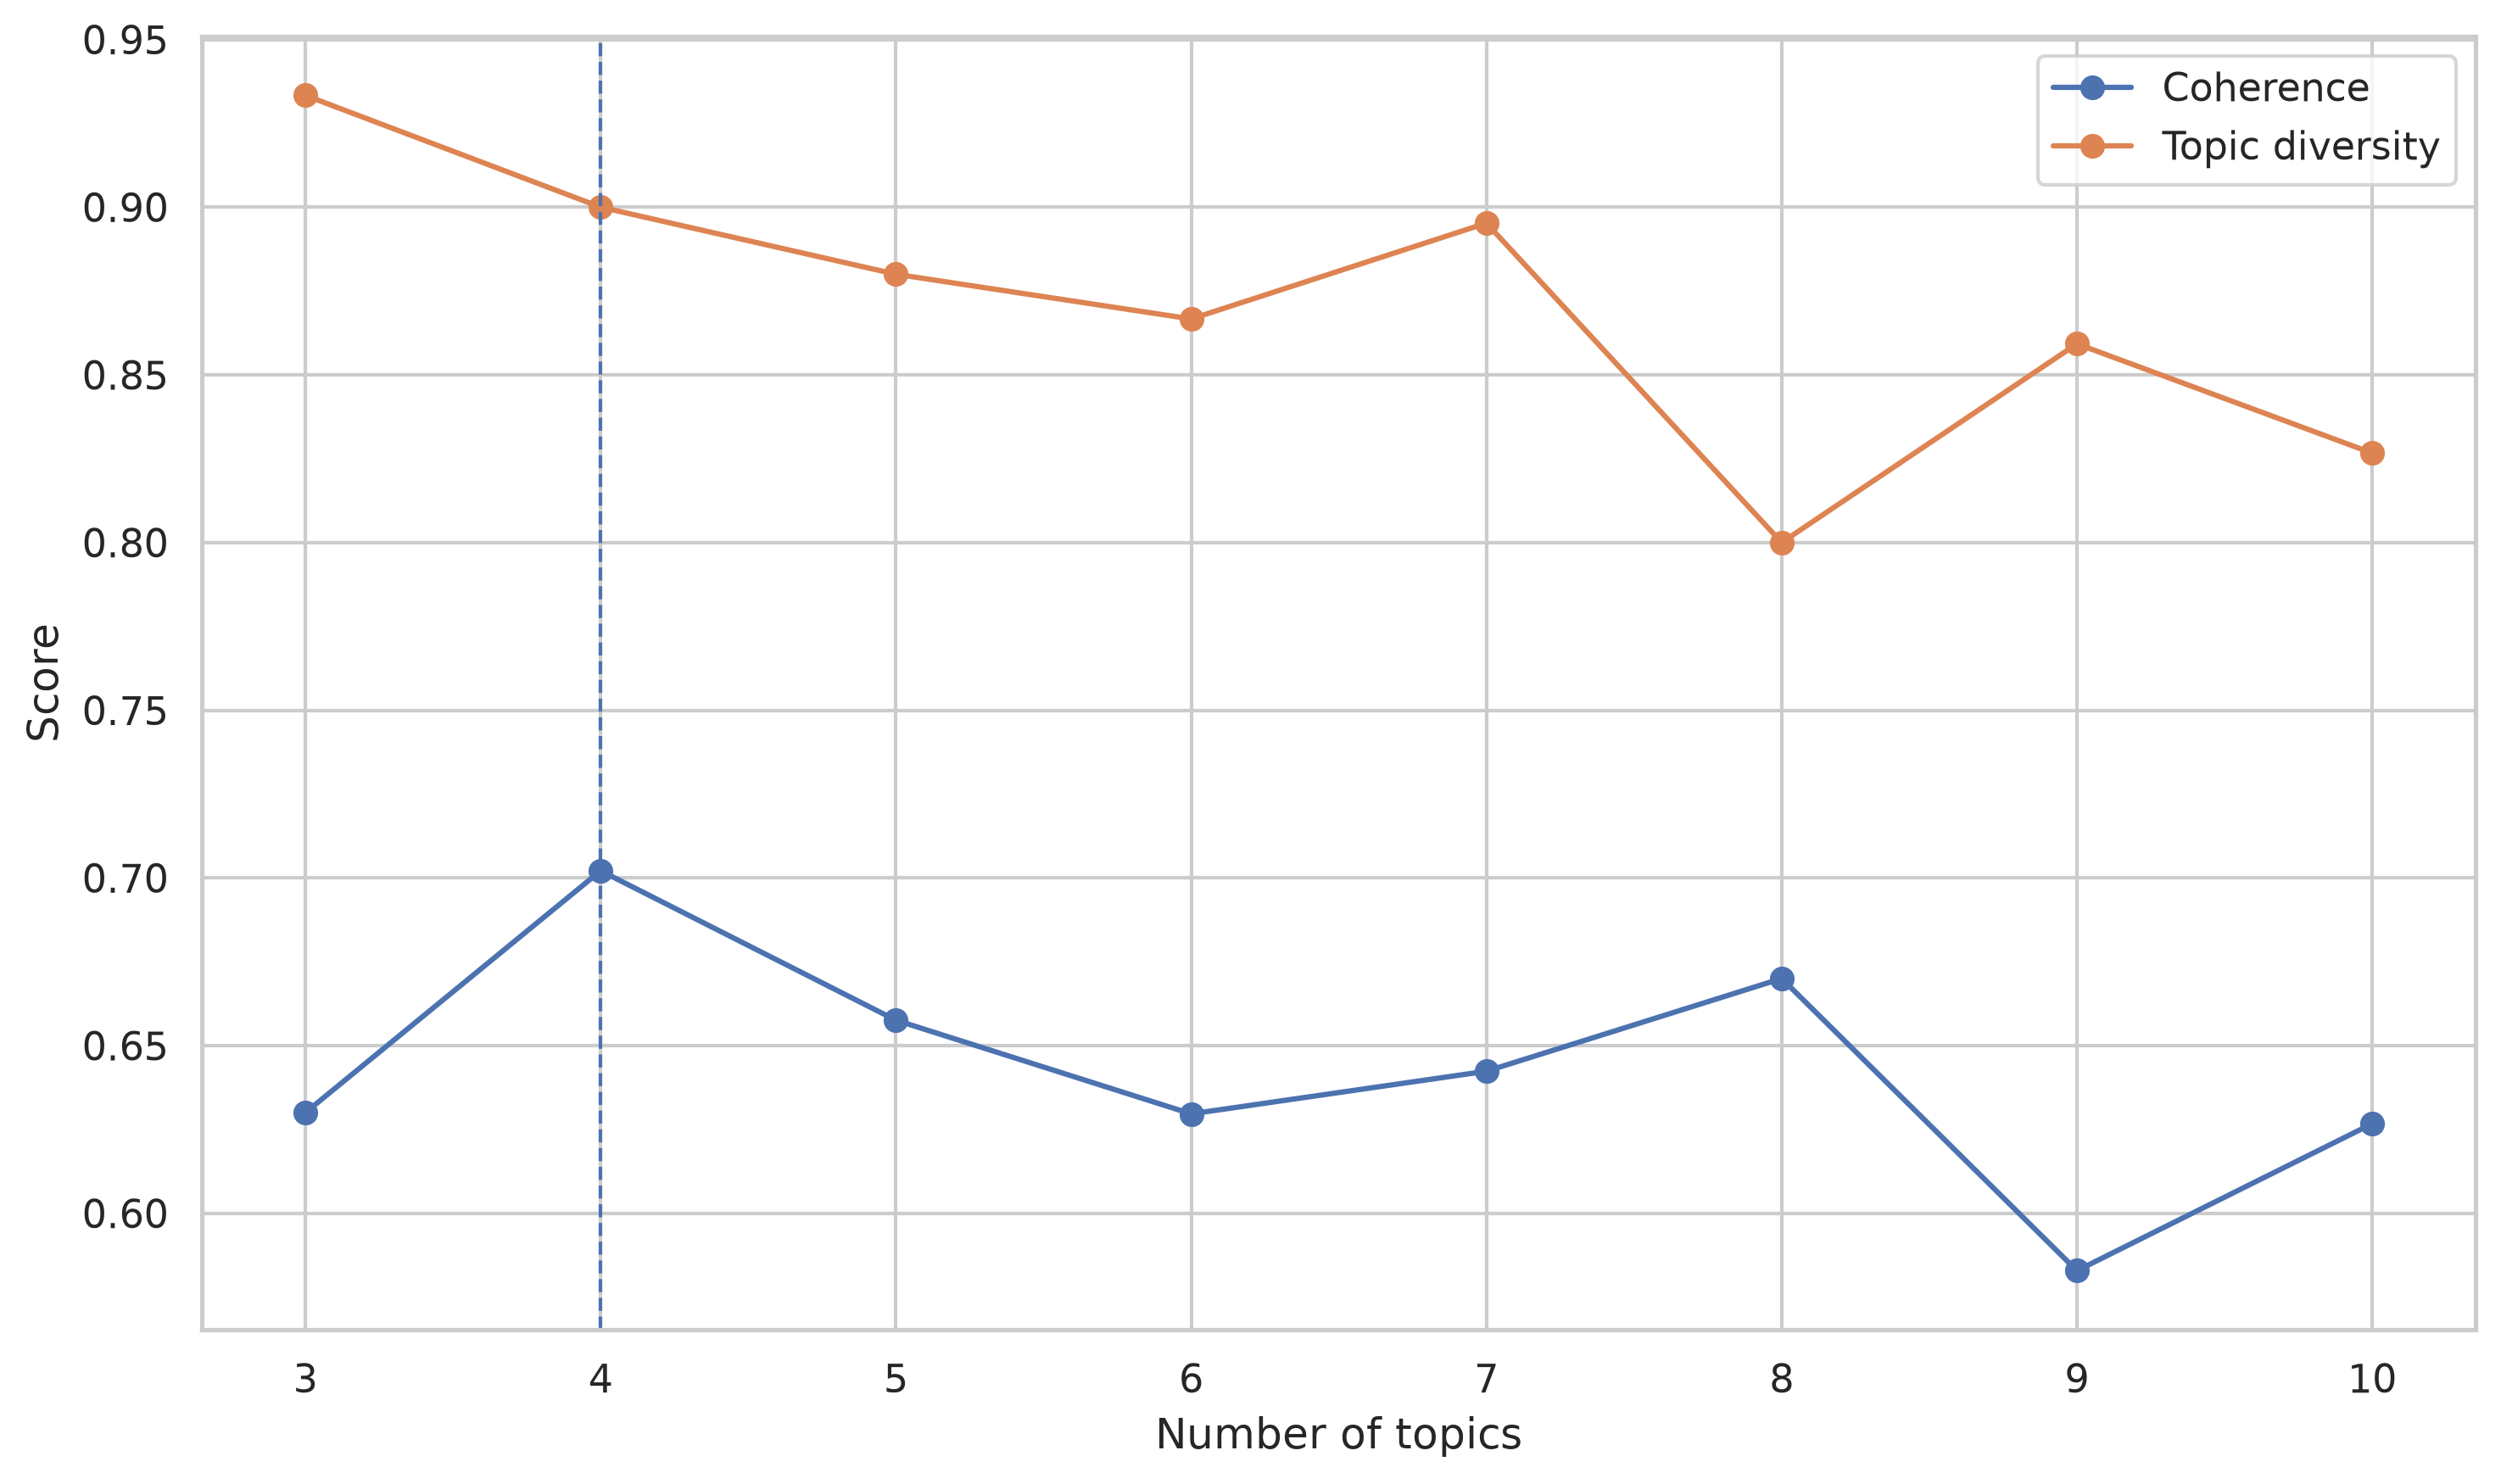
\includegraphics[scale=.45]{images/lda_policy_global_coherence_diversity.png}
    \caption{Global policy LDA topic-number search using coherence and diversity.}
    \label{fig:lda-policy-global-search}
\end{figure}

\begin{table}[t]
\centering
\small
\begin{tabular}{p{0.10\linewidth}p{0.78\linewidth}}
\hline
Topic & Main terms \\
\hline
0 & privacy, staff, content, educator, bias, guidance, decision, potential, principle, risk \\
1 & competency, knowledge, skill, curriculum, social, framework, professional, ethic, pedagogical \\
2 & child, strategy, framework, literacy, research, public, guidance, learner, regulation \\
3 & usage, outils, cadre, donn\'{e}es, p\'{e}dagogique, num\'{e}rique, utilisation, d\'{e}ploiement \\
\hline
\end{tabular}
\caption{Global policy LDA topics. The fourth topic reflects French-language policy material and is kept as part of the corpus rather than translated away.}
\label{tab:lda-policy-global-topics}
\end{table}

Country-specific LDA models were also fitted to inspect whether the global themes
were expressed differently across national policy corpora. Australia showed signals
around assessment, privacy, academic integrity and policy risk. France emphasised
strategy, research, innovation and education deployment. Ireland was associated with
regulation, safety, teaching, assessment and literacy. The USA showed signals around
privacy, bias, equity, assessment and practical guidance. These results support the
use of LDA as an initial map, but they also show why a more refined topic model is
needed later: several LDA topics still mix governance language, education-practice
language and institutional reporting language in the same component.

\subsection{Sentiment LDA pipeline and synthetic-data stress test}

The sentiment LDA pipeline\footnote{\href{https://github.com/nsirimai/mscdsa/blob/main/msc/progress/topic_modelling/lda/sentiment/lda_topic_modelling.ipynb}{\texttt{github.com/nsirimai/mscdsa/blob/main/msc/progress/topic\_modelling/lda/sentiment/lda\_topic\_modelling.ipynb}}} was used differently from the policy pipeline. Here,
synthetic sentiment data was introduced deliberately as a robustness stress test. The
objective was not to enlarge the corpus for final evidence, but to test whether
artificial text can shift or corrupt the topic structure. This distinction is
important because synthetic text can be useful in limited-data settings, but only
when it is clearly identified, kept analytically separate from empirical observations
and evaluated for downstream effects
\cite{halterman2025synthetic,chen2023empirical,chim2025evaluating}.

\begin{verbatim}
Original sentiment data
  -> add synthetic data deliberately for stress testing
  -> clean and preprocess text
  -> build dictionary and document-term matrix
  -> search LDA topic numbers using coherence and diversity
  -> compare original and synthetic topic structures
  -> check whether new topic signals appear
\end{verbatim}

\begin{figure}[h]
    \centering
    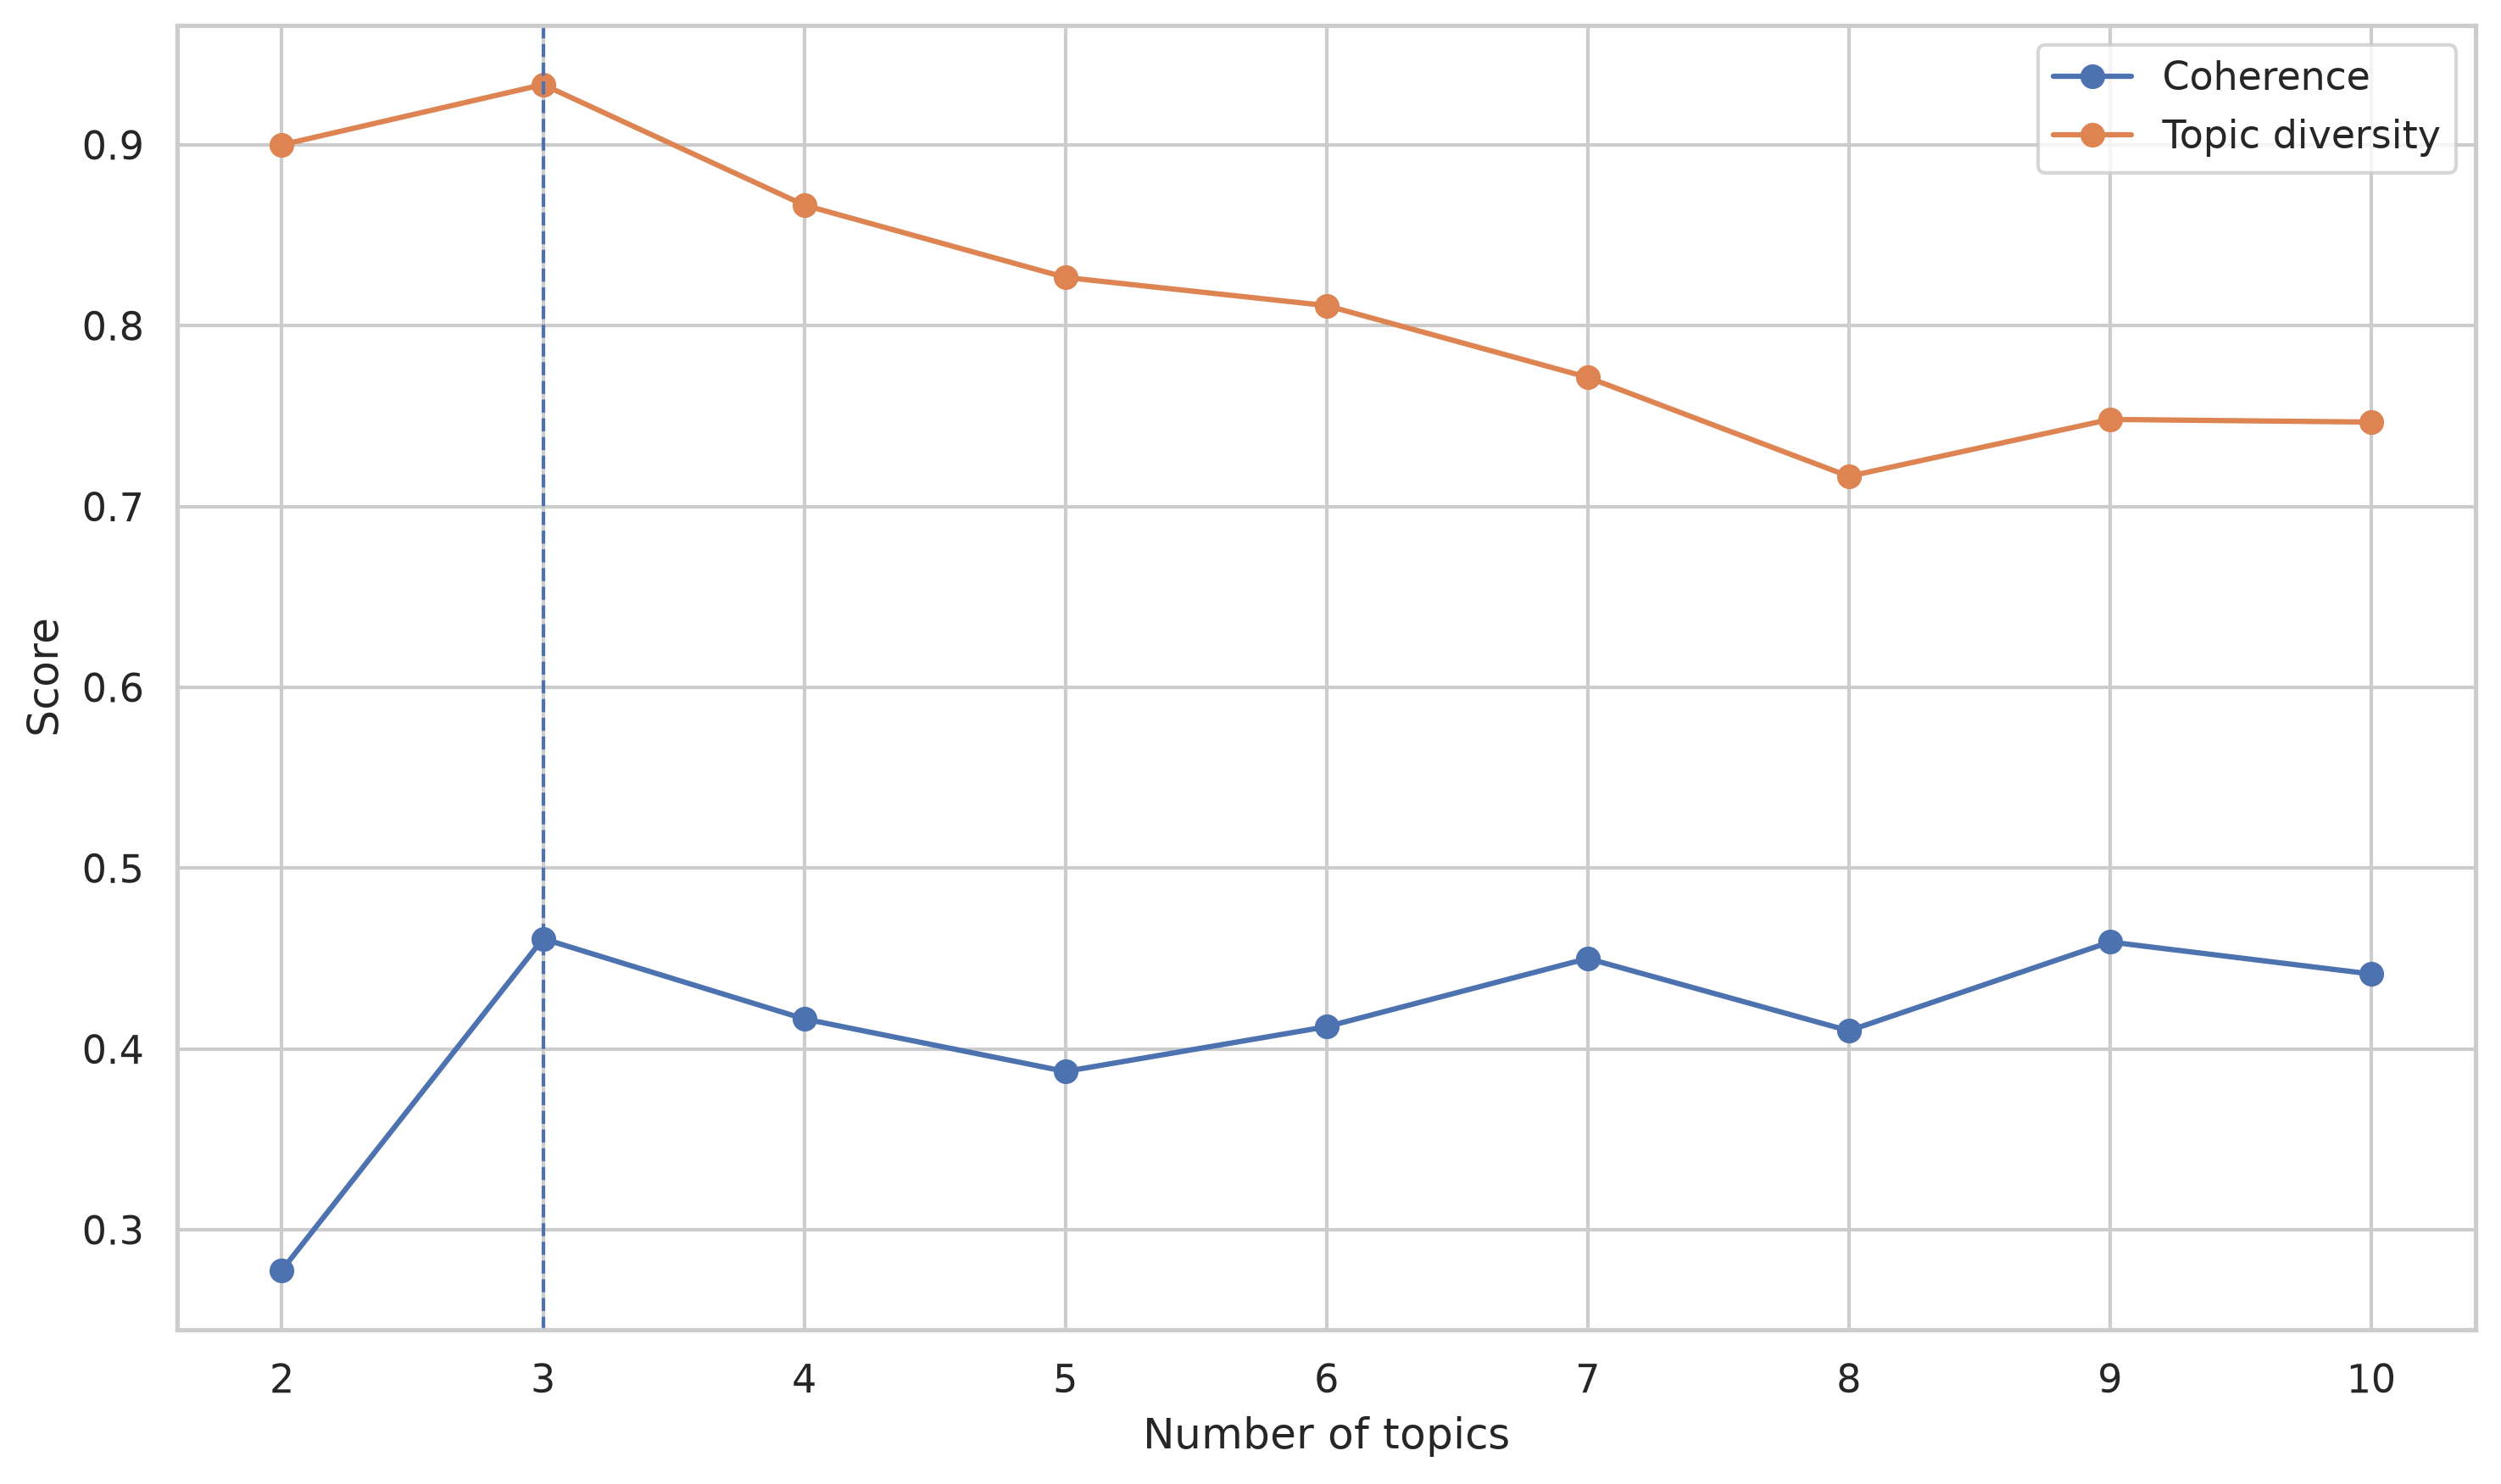
\includegraphics[scale=.45]{images/lda_sentiment_original_coherence_diversity.png}
    \caption{LDA topic-number search on original sentiment chunks.}
    \label{fig:lda-sentiment-original-search}
\end{figure}

\begin{table}[h]
\centering
\small
\begin{tabular}{p{0.22\linewidth}p{0.18\linewidth}p{0.48\linewidth}}
\hline
Subset & Best topics & Main signal \\
\hline
Original sentiment & 3 & ethics, skills, social perception, experience, learning pathways \\
Synthetic sentiment & 4 & protection, negative sentiment, integrity, access, fear, trust, governance \\
\hline
\end{tabular}
\caption{Separate LDA topic searches for original and synthetic sentiment chunks. The synthetic subset changes the topic structure and is therefore treated as robustness data, not empirical evidence.}
\label{tab:lda-sentiment-original-synthetic}
\end{table}

The original sentiment corpus contained 17 documents and 498 chunks, while the
synthetic sentiment corpus contained 53 documents and 211 chunks. When modelled
separately, the original sentiment subset selected three topics (see
Figure~\ref{fig:lda-sentiment-original-search}), whereas the synthetic subset
selected four topics. This was a key methodological finding: synthetic data did not
simply reinforce the original themes; it introduced an additional topic structure.
The original sentiment topics were centred on ethics, skills, social perception,
experience and learning pathways. By contrast, the synthetic subset amplified signals
around protection, negative sentiment, integrity, access, fear, trust and governance.
Table~\ref{tab:lda-sentiment-original-synthetic} summarises this difference.


This result motivates a strict rule used in the rest of the topic-modelling work:
synthetic sentiment chunks are allowed for robustness and sensitivity checks, but
they are not allowed to define the final empirical topic structure. Synthetic data is
used to test whether the pipeline is stable under artificial perturbation; it is not
used to claim new facts about real public opinion.

\subsection{Limitations and transition to later topic models}

The LDA baseline is transparent, reproducible and easy to inspect, but it remains
limited for this project. Its bag-of-words representation does not capture contextual
semantic similarity, and policy chunks often mix governance, institutional and
education-practice language in the same passage. The sentiment stress test also shows
that topic discovery can be sensitive to synthetic text.

These limits motivate the next comparison. BERTopic is used to test whether
embedding-based semantic clustering changes the thematic structure, while NMF is used
as the main reference model because it produces stable topic--word and
document--topic matrices that are easier to inspect, aggregate and compare across the
policy and sentiment corpora.

\section{BERTopic as a semantic-clustering baseline}

After the LDA baseline, BERTopic was used as a second topic-discovery pipeline for
both the policy and sentiment corpora. Unlike LDA, BERTopic treats topic modelling as
a clustering problem: documents are embedded, grouped into clusters, and then
represented through class-based TF--IDF topic terms~\cite{grootendorst2022bertopic}.
In this implementation, cleaned policy and sentiment chunks were converted into
TF--IDF/SVD document embeddings before clustering, and topic keywords were extracted
with the BERTopic representation layer. This kept the pipeline close to the cleaned
lexical evidence used in LDA, while still testing whether a clustering-based model
produces a different thematic structure.

\begin{verbatim}
Cleaned chunks
  -> TF--IDF vocabulary and SVD document embeddings
  -> search candidate BERTopic topic numbers
  -> evaluate coherence, cosine silhouette and topic balance
  -> fit the selected global model
  -> extract topic keywords and representative documents
  -> use a small language model only for topic phrasing
\end{verbatim}

The number of topics was again selected as a model-selection problem. Topic coherence
was retained to measure whether each topic produced meaningful word groups
\cite{roder2015exploring}. Cosine silhouette was added because BERTopic is a
clustering-based method, and silhouette analysis measures whether documents are
closer to their assigned cluster than to other clusters. Topic balance was used as an
internal diagnostic to penalise models dominated by a single large topic. The final
selection score combined these criteria, so the chosen model had to be interpretable,
separated and not too imbalanced.

\subsection{Policy BERTopic outcome}

For the global policy corpus, the BERTopic search selected nine topics. The selected
model had coherence 0.1060, cosine silhouette 0.1370, a largest topic share of 0.204
and a smallest topic share of 0.038. Figure~\ref{fig:bertopic-policy-combined}
shows the topic-number search on the left and the country-level topic distribution on
the right. Although the ten-topic model achieved slightly higher coherence and
balance, the nine-topic model obtained the strongest combined selection score because
it gave the best separation while avoiding excessive fragmentation, as shown in
Table~\ref{tab:bertopic-policy-global-topics}.

\begin{figure}[h]
    \centering
    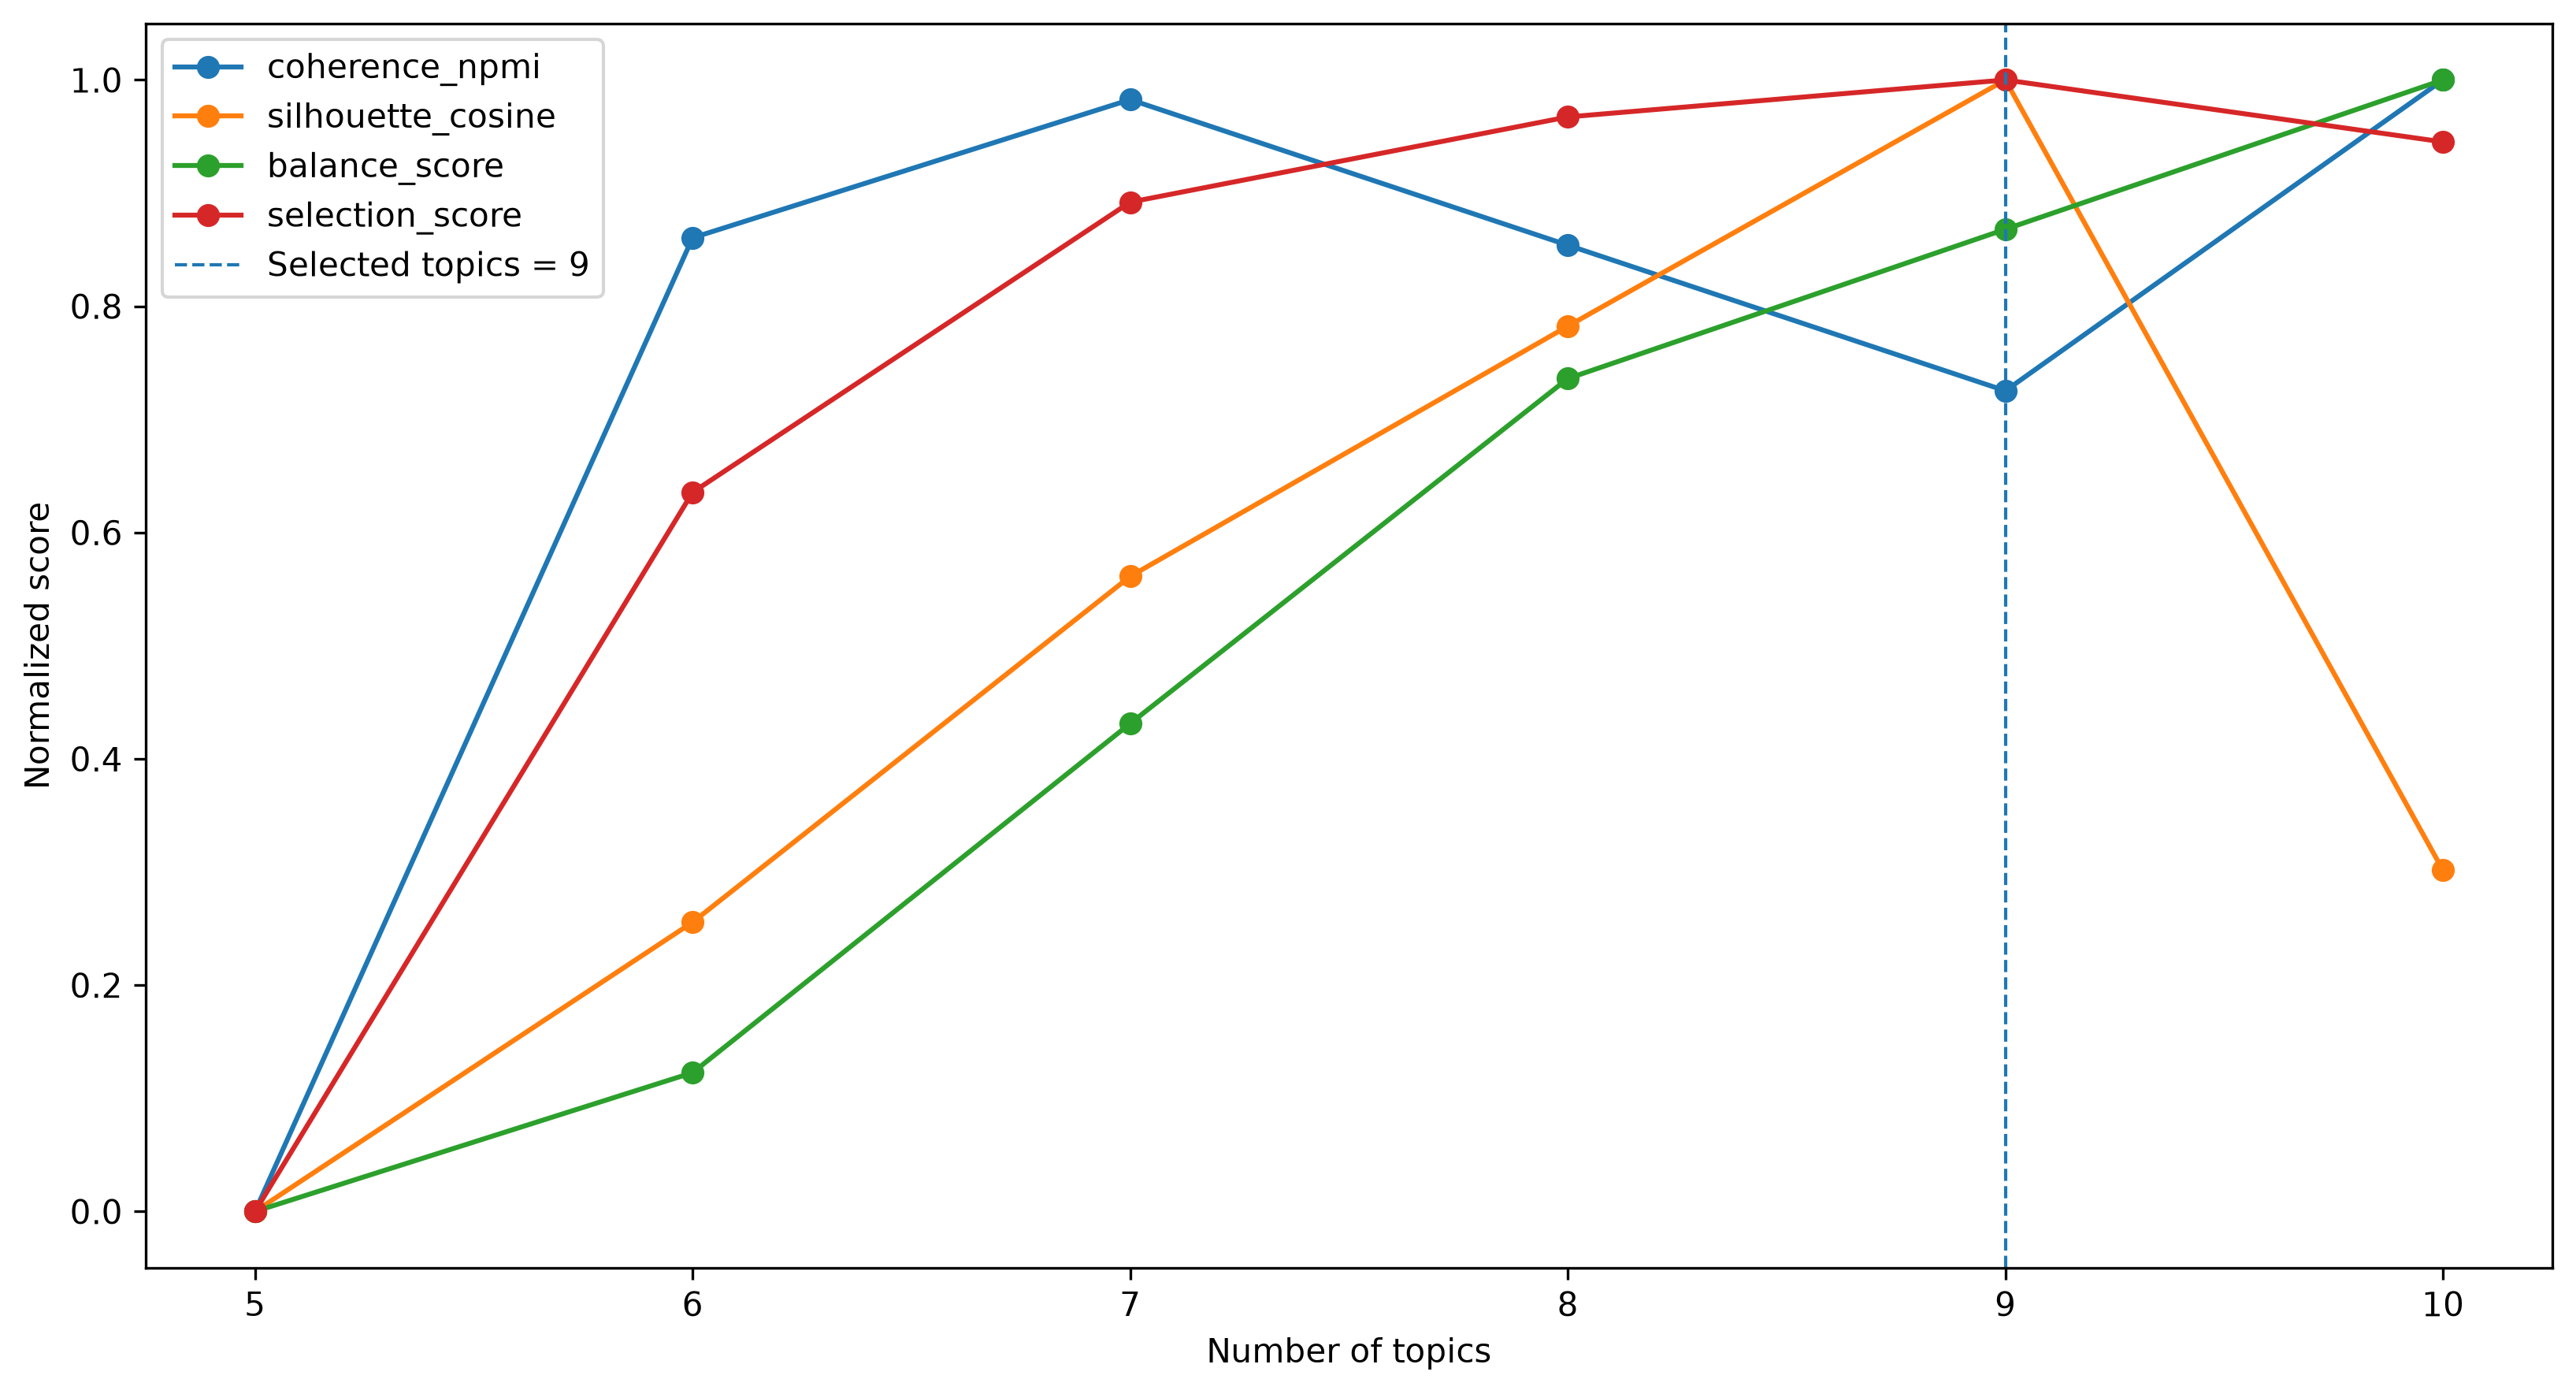
\includegraphics[scale=.29]{images/bert_policy_global_topic_selection_metrics.png}
    \hspace{0.04\linewidth}
    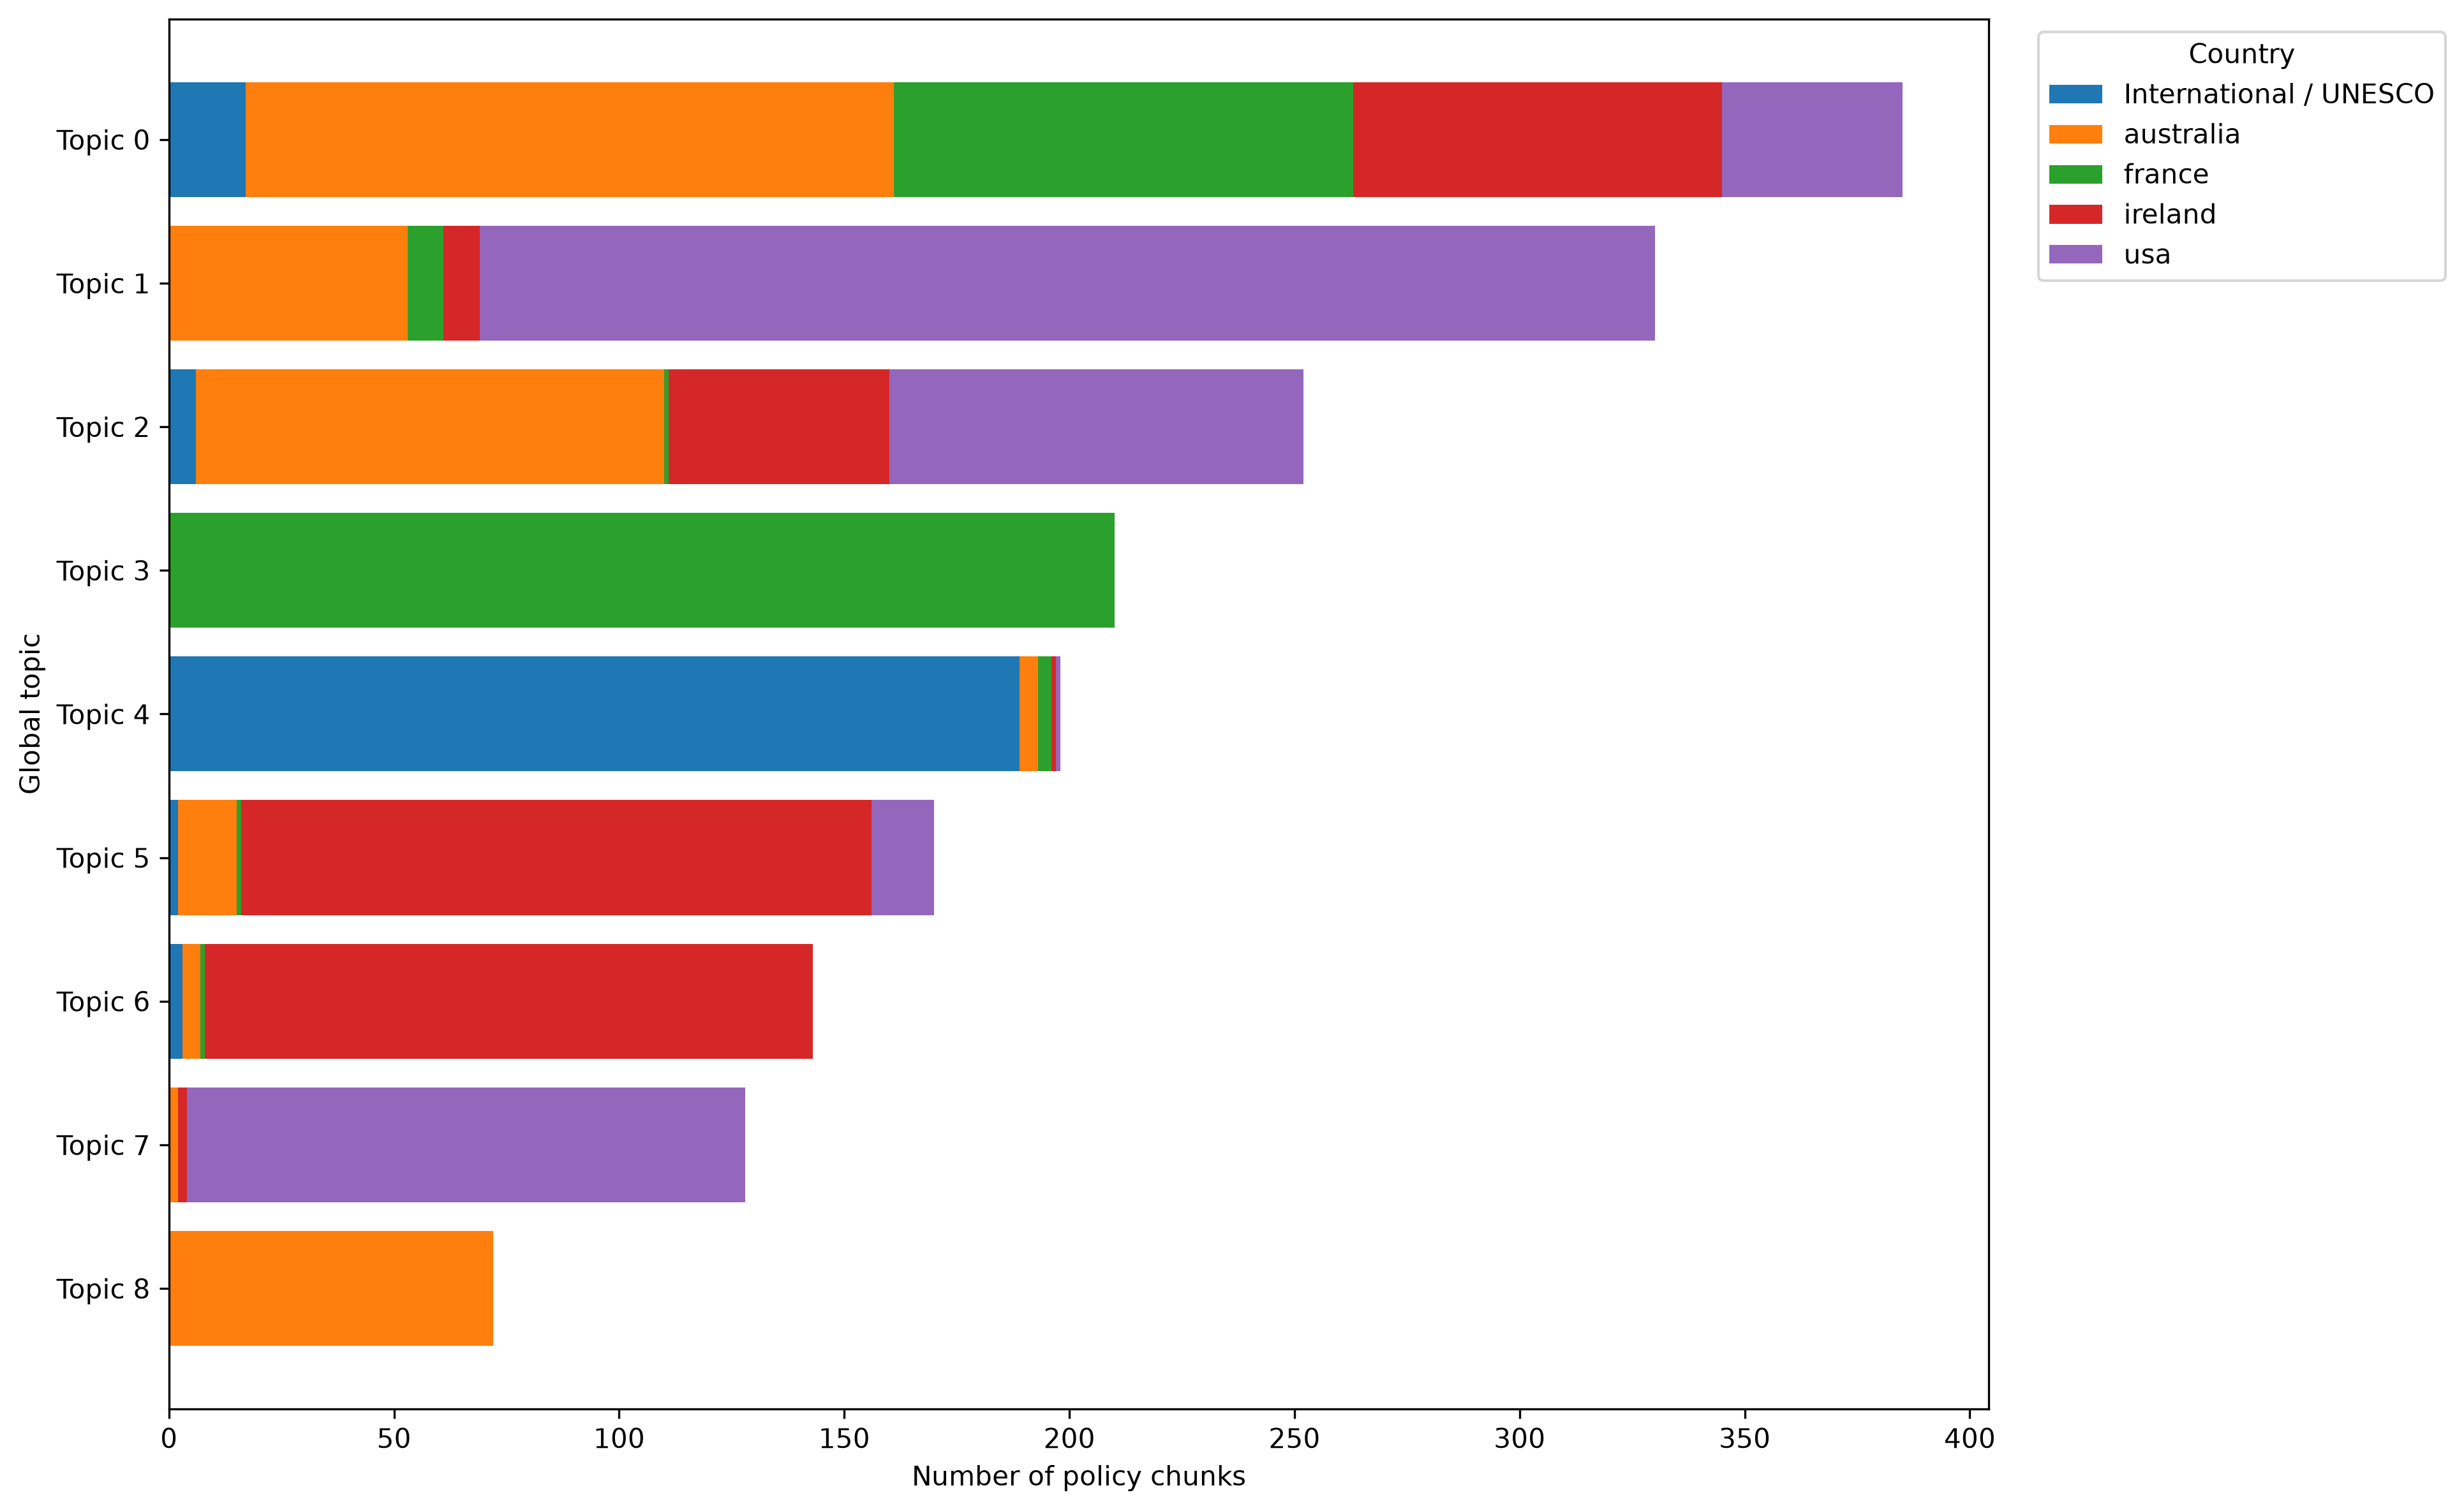
\includegraphics[scale=.225]{images/bert_policy_global_topic_distribution_by_country.png}

    \caption{Policy BERTopic results. Left: topic-number search using normalised coherence, cosine silhouette, balance and the combined selection score. Right: distribution of global policy BERTopic topics by country.}
    \label{fig:bertopic-policy-combined}
\end{figure}

\begin{table}[h]
\centering
\small
\begin{tabular}{p{0.10\linewidth}p{0.16\linewidth}p{0.58\linewidth}}
\hline
Topic & Share & SLM topic phrase \\
\hline
0 & 0.204 & AI curriculum integration and oversight \\
1 & 0.175 & AI-assisted instructional policies \\
2 & 0.133 & Educational AI usage policies \\
3 & 0.111 & AI in school curriculum and teacher training \\
4 & 0.105 & Competency-based education and assessment \\
5 & 0.090 & AI child protection and rights oversight \\
6 & 0.076 & Digital learning progression framework \\
7 & 0.068 & AI in education and student achievement \\
8 & 0.038 & AI offloading and metacognitive skills in education \\
\hline
\end{tabular}
\caption{Global policy BERTopic topics after SLM phrasing. The SLM is used only to phrase discovered topics, not to create the topic assignments.}
\label{tab:bertopic-policy-global-topics}
\end{table}


\begin{table}[h]
\centering
\small
\begin{tabular}{p{0.10\linewidth}p{0.16\linewidth}p{0.58\linewidth}}
\hline
Topic & Share & SLM topic phrase \\
\hline
0 & 0.207 & Concern over AI usage in education \\
1 & 0.147 & Teacher adaptation and classroom AI use \\
2 & 0.125 & Impact of learning experience on knowledge and skills \\
3 & 0.116 & Ethics framework development for AI in education \\
4 & 0.116 & Concerns and risks around AI in education \\
5 & 0.097 & Concern over AI risks and social harm \\
6 & 0.066 & Concerns over GenAI implementation in education \\
7 & 0.064 & Public opinion on AI fears and hopes \\
8 & 0.062 & Concern over AI risks and benefits \\
\hline
\end{tabular}
\caption{Original sentiment BERTopic topics after SLM phrasing. The labels are generated after clustering and are used for readability only.}
\label{tab:bertopic-sentiment-topics}
\end{table}

The global topics remained centred on AI in education policy, but they were more
fine-grained than the LDA baseline. Instead of one broad governance/education
mixture, BERTopic separated curriculum integration, instructional use, student
achievement, child protection, competency frameworks and metacognitive skills. The
country-level distribution shown on the right of
Figure~\ref{fig:bertopic-policy-combined} was used to inspect whether these global
topics were expressed differently across national policy sources.

Country-specific BERTopic models were also fitted as a secondary check. Australia and
Ireland selected four topics, France selected eight topics and the USA selected nine
topics. This confirmed that the same global policy vocabulary is not distributed
uniformly across the national corpora: some countries produce compact topic structures,
whereas others require more granular models.

\subsection{Sentiment BERTopic outcome and synthetic robustness}

The sentiment BERTopic pipeline used the same modelling logic, but synthetic data was
used only as a robustness tool. The original sentiment chunks were used to fit the
empirical BERTopic model. Synthetic sentiment chunks were then assigned to the
learned topic space in order to test whether the discovered structure was stable
under artificial perturbation. This follows the same rule introduced in the LDA
stage: synthetic text can support stress testing and data augmentation research, but
it must be kept analytically separate from empirical evidence
\cite{halterman2025synthetic,chen2023empirical,chim2025evaluating}.

For the original sentiment corpus, the topic-number search selected nine topics. The
selected model had coherence 0.0538, cosine silhouette 0.1418, a largest topic share
of 0.231 and balance 0.769. Figure~\ref{fig:bertopic-sentiment-search} shows why the
nine-topic model was retained: the ten-topic model had slightly stronger silhouette
and balance, but the nine-topic model produced the highest combined selection score
because it was substantially more coherent. The resulting sentiment topics mainly
capture concern, teacher adaptation, learning experience, ethics, implementation
risks, social harm and public hopes or fears around AI in education. The topic shares
and SLM-generated phrases are summarised in
Table~\ref{tab:bertopic-sentiment-topics}. This provides a more fine-grained
sentiment map than the LDA baseline while preserving topic-level interpretability.

\begin{figure}[h]
    \centering
    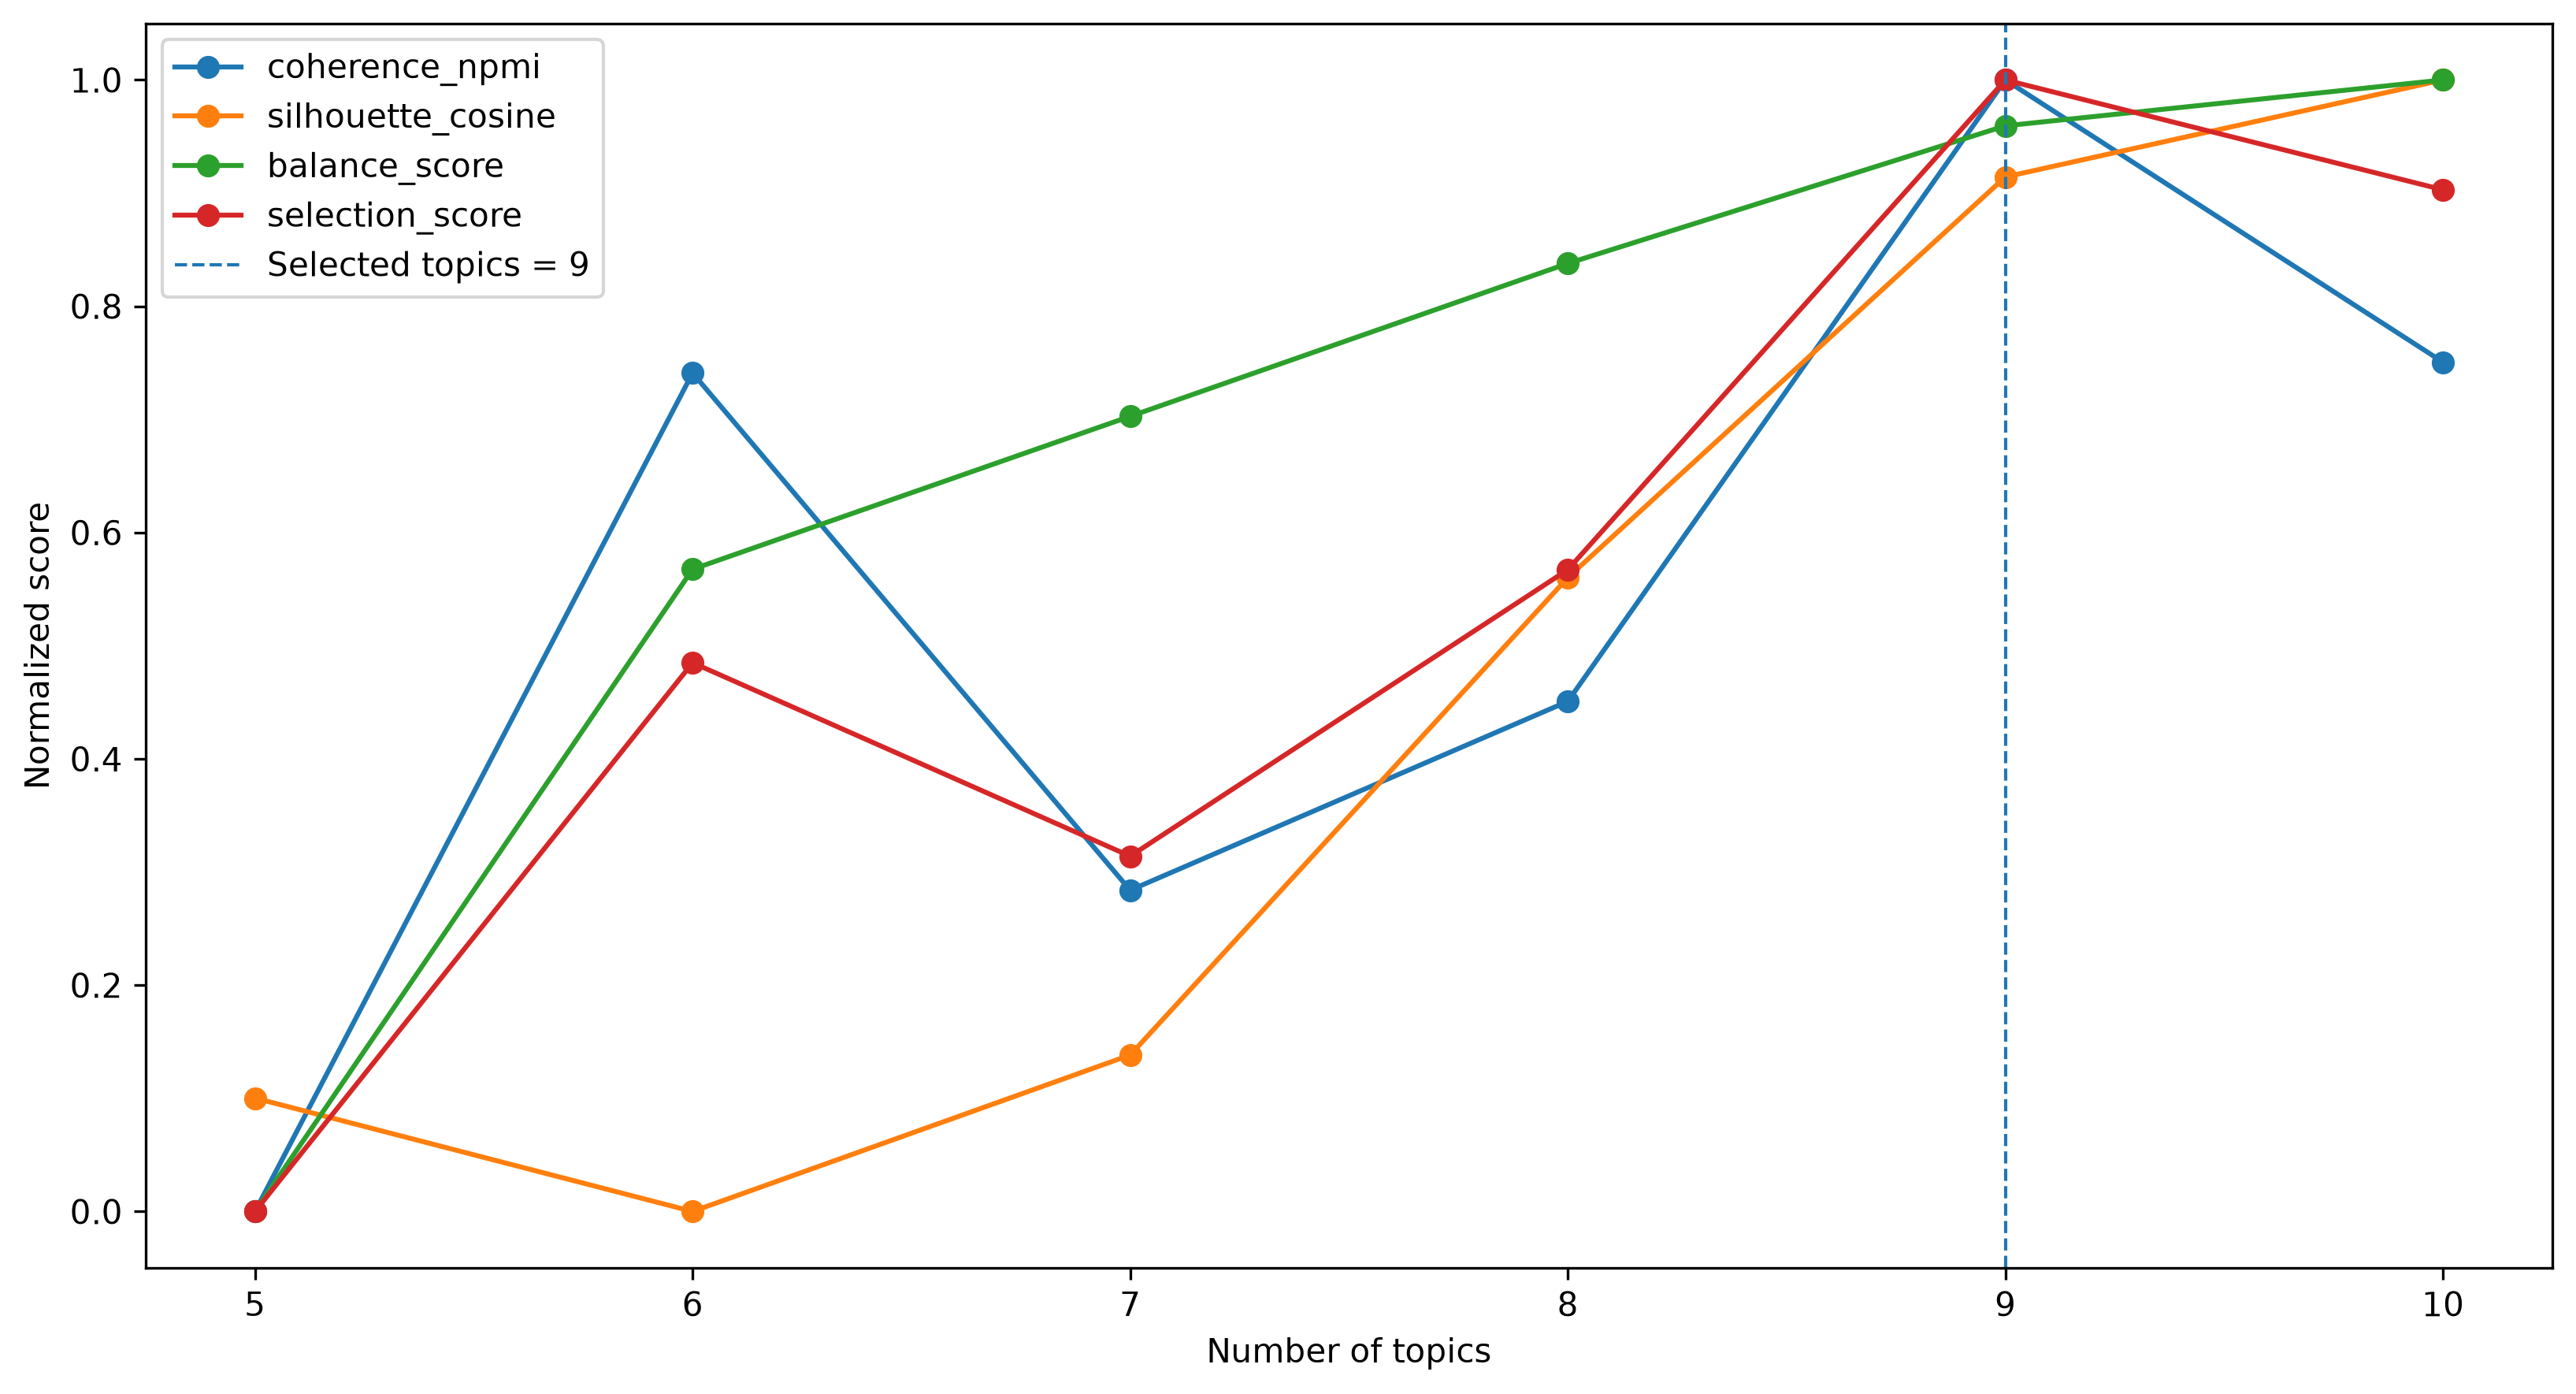
\includegraphics[scale=0.4]{images/bert_sentiment_topic_selection_metrics.png}
    \caption{Sentiment BERTopic topic-number search using normalised coherence, cosine silhouette, balance and the combined selection score.}
    \label{fig:bertopic-sentiment-search}
\end{figure}



The SLM phrasing layer was added to improve readability of the output tables and
figures. For each topic, the SLM received the top keywords and a small number of
representative chunks, and returned a short topic label, a prototype sentence and a
coherence flag. This is used as an interpretation layer only. The topic model still
defines the assignments, distributions and robustness checks. This separation reduces
the risk of letting a generative model rewrite the empirical structure while still
using it for clearer presentation of topic meaning
\cite{gilardi2023chatgpt,ziems2024llms}.

The synthetic robustness report showed that synthetic chunks did not distribute
evenly across the learned sentiment topics. Figure~\ref{fig:bertopic-sentiment-synthetic-combined} (Left)
compares the original and synthetic topic shares. Some original topics received no
synthetic chunks, while topics related to GenAI implementation, public fears and
general AI risk were over-represented. This confirms that synthetic data is useful as
a robustness probe, but it should not be merged with the original sentiment corpus to
define the final empirical topic structure.

\begin{figure}[h]
    \centering
    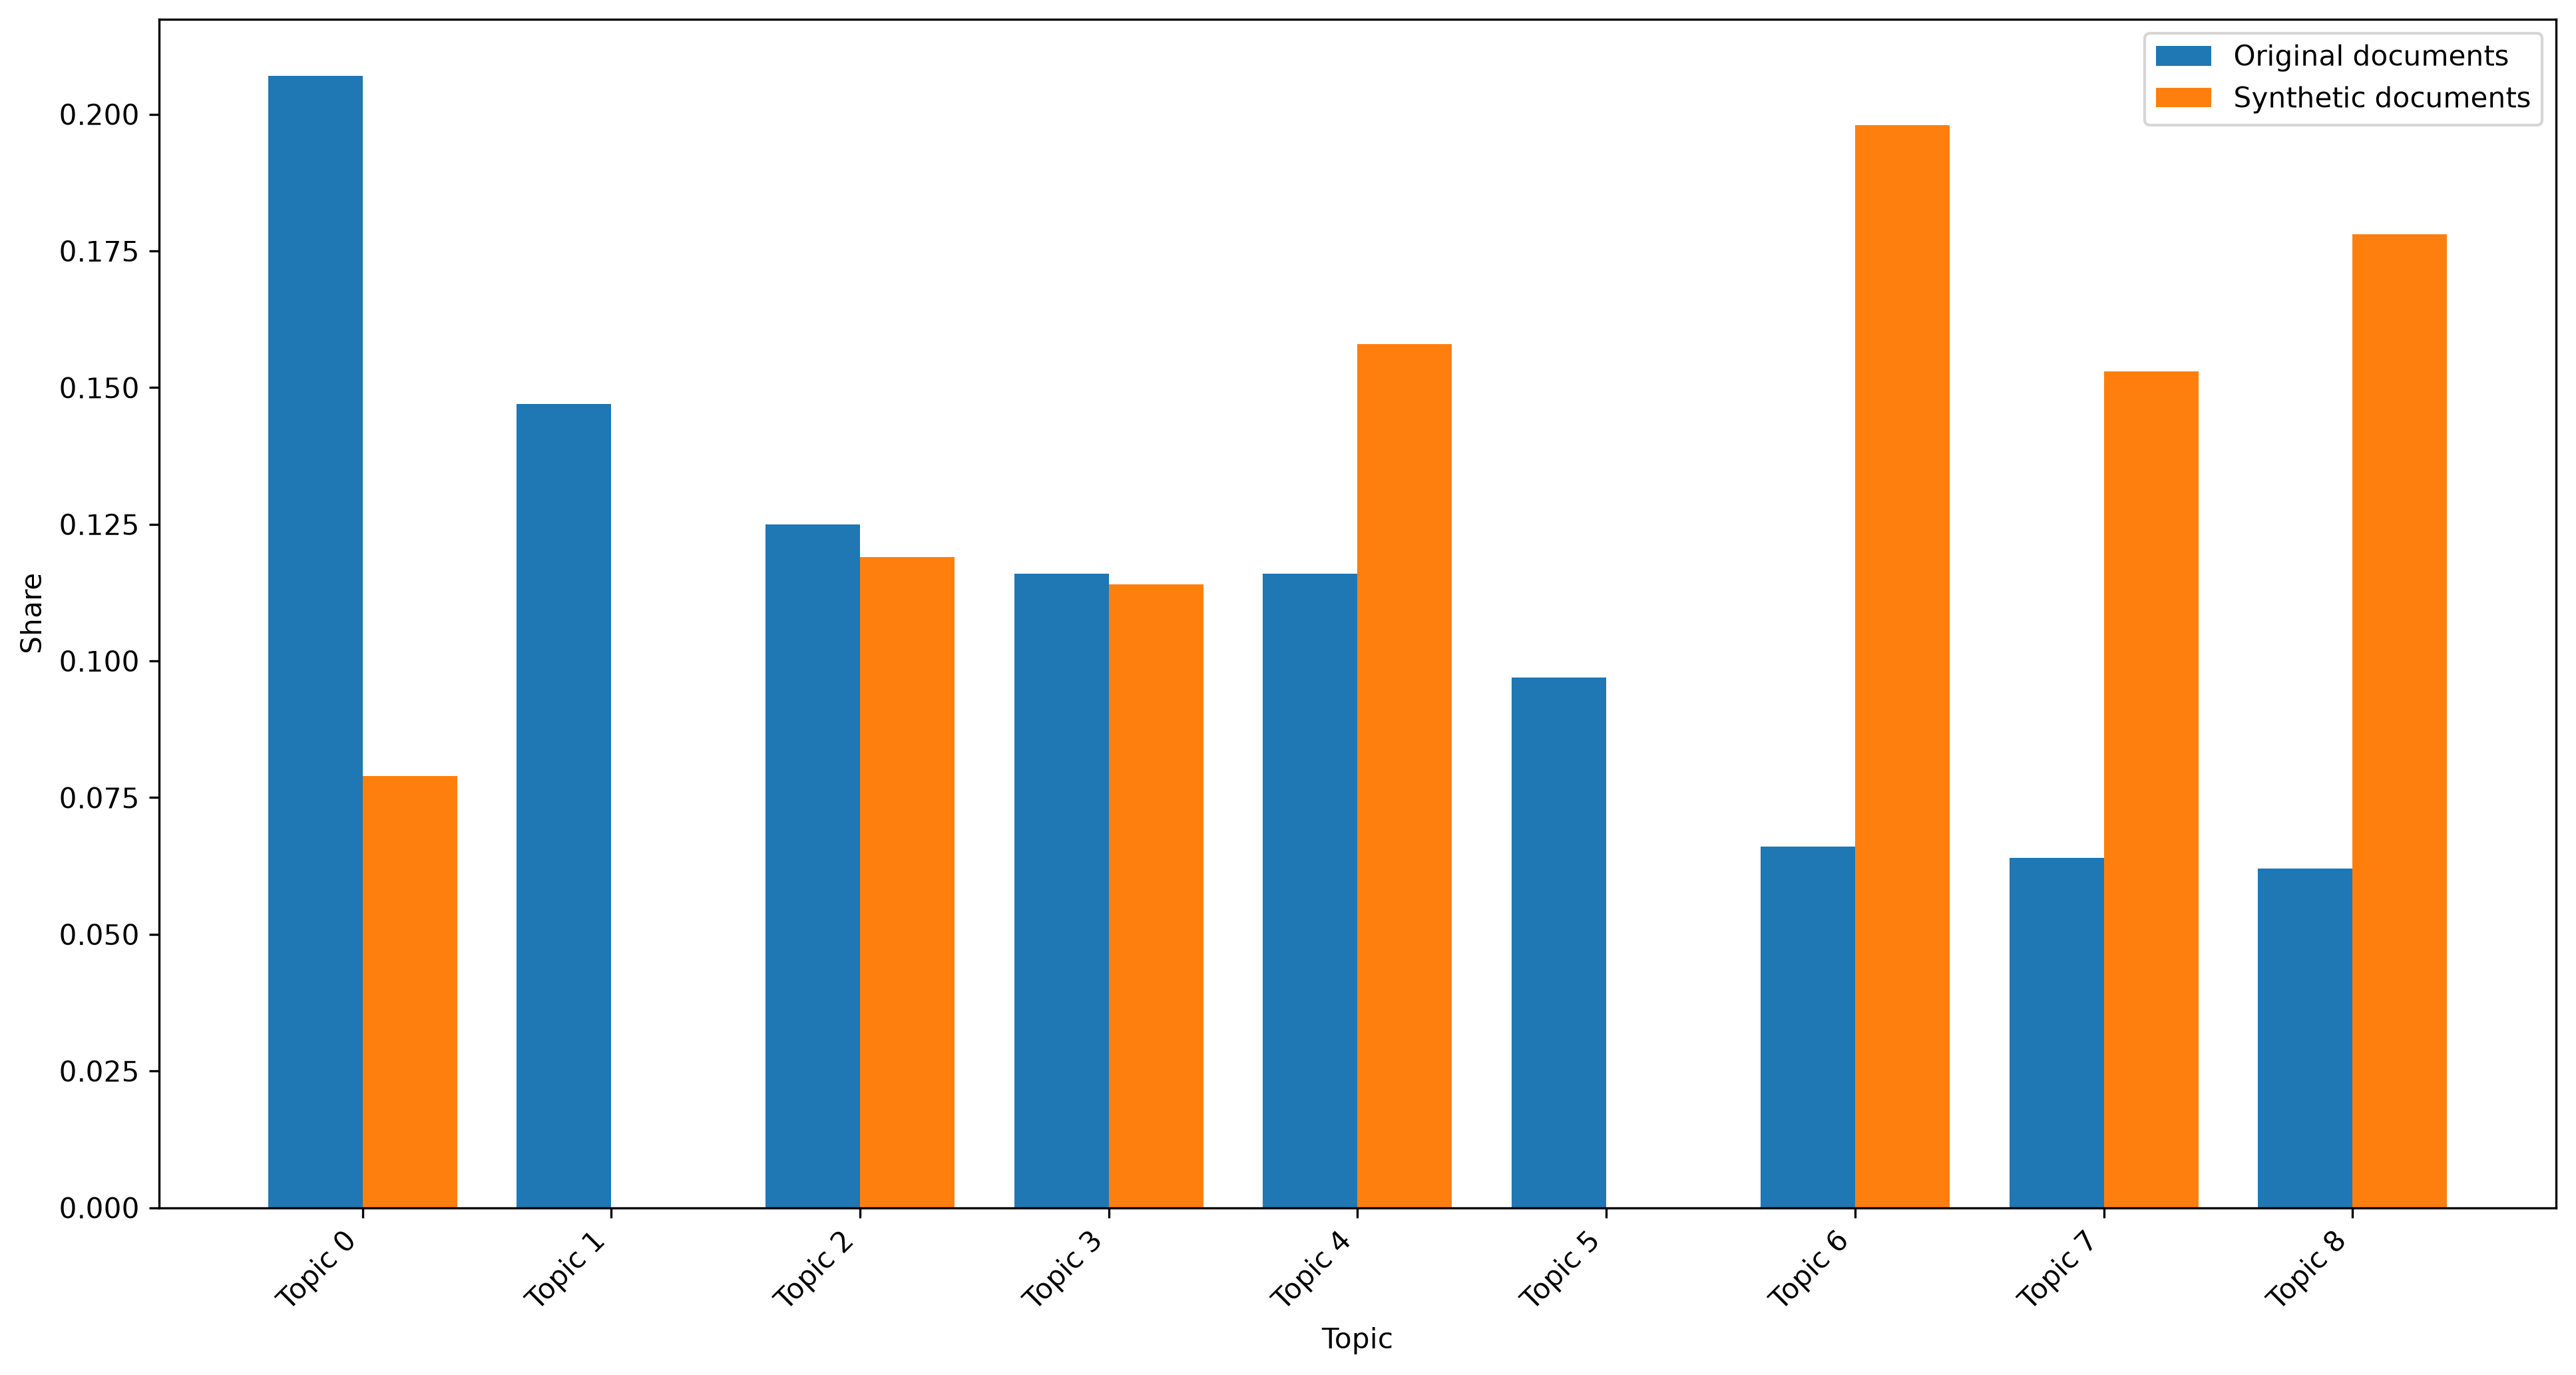
\includegraphics[scale=.23]{images/bert_sentiment_original_vs_synthetic_distribution.png}
    \hspace*{.1cm}
    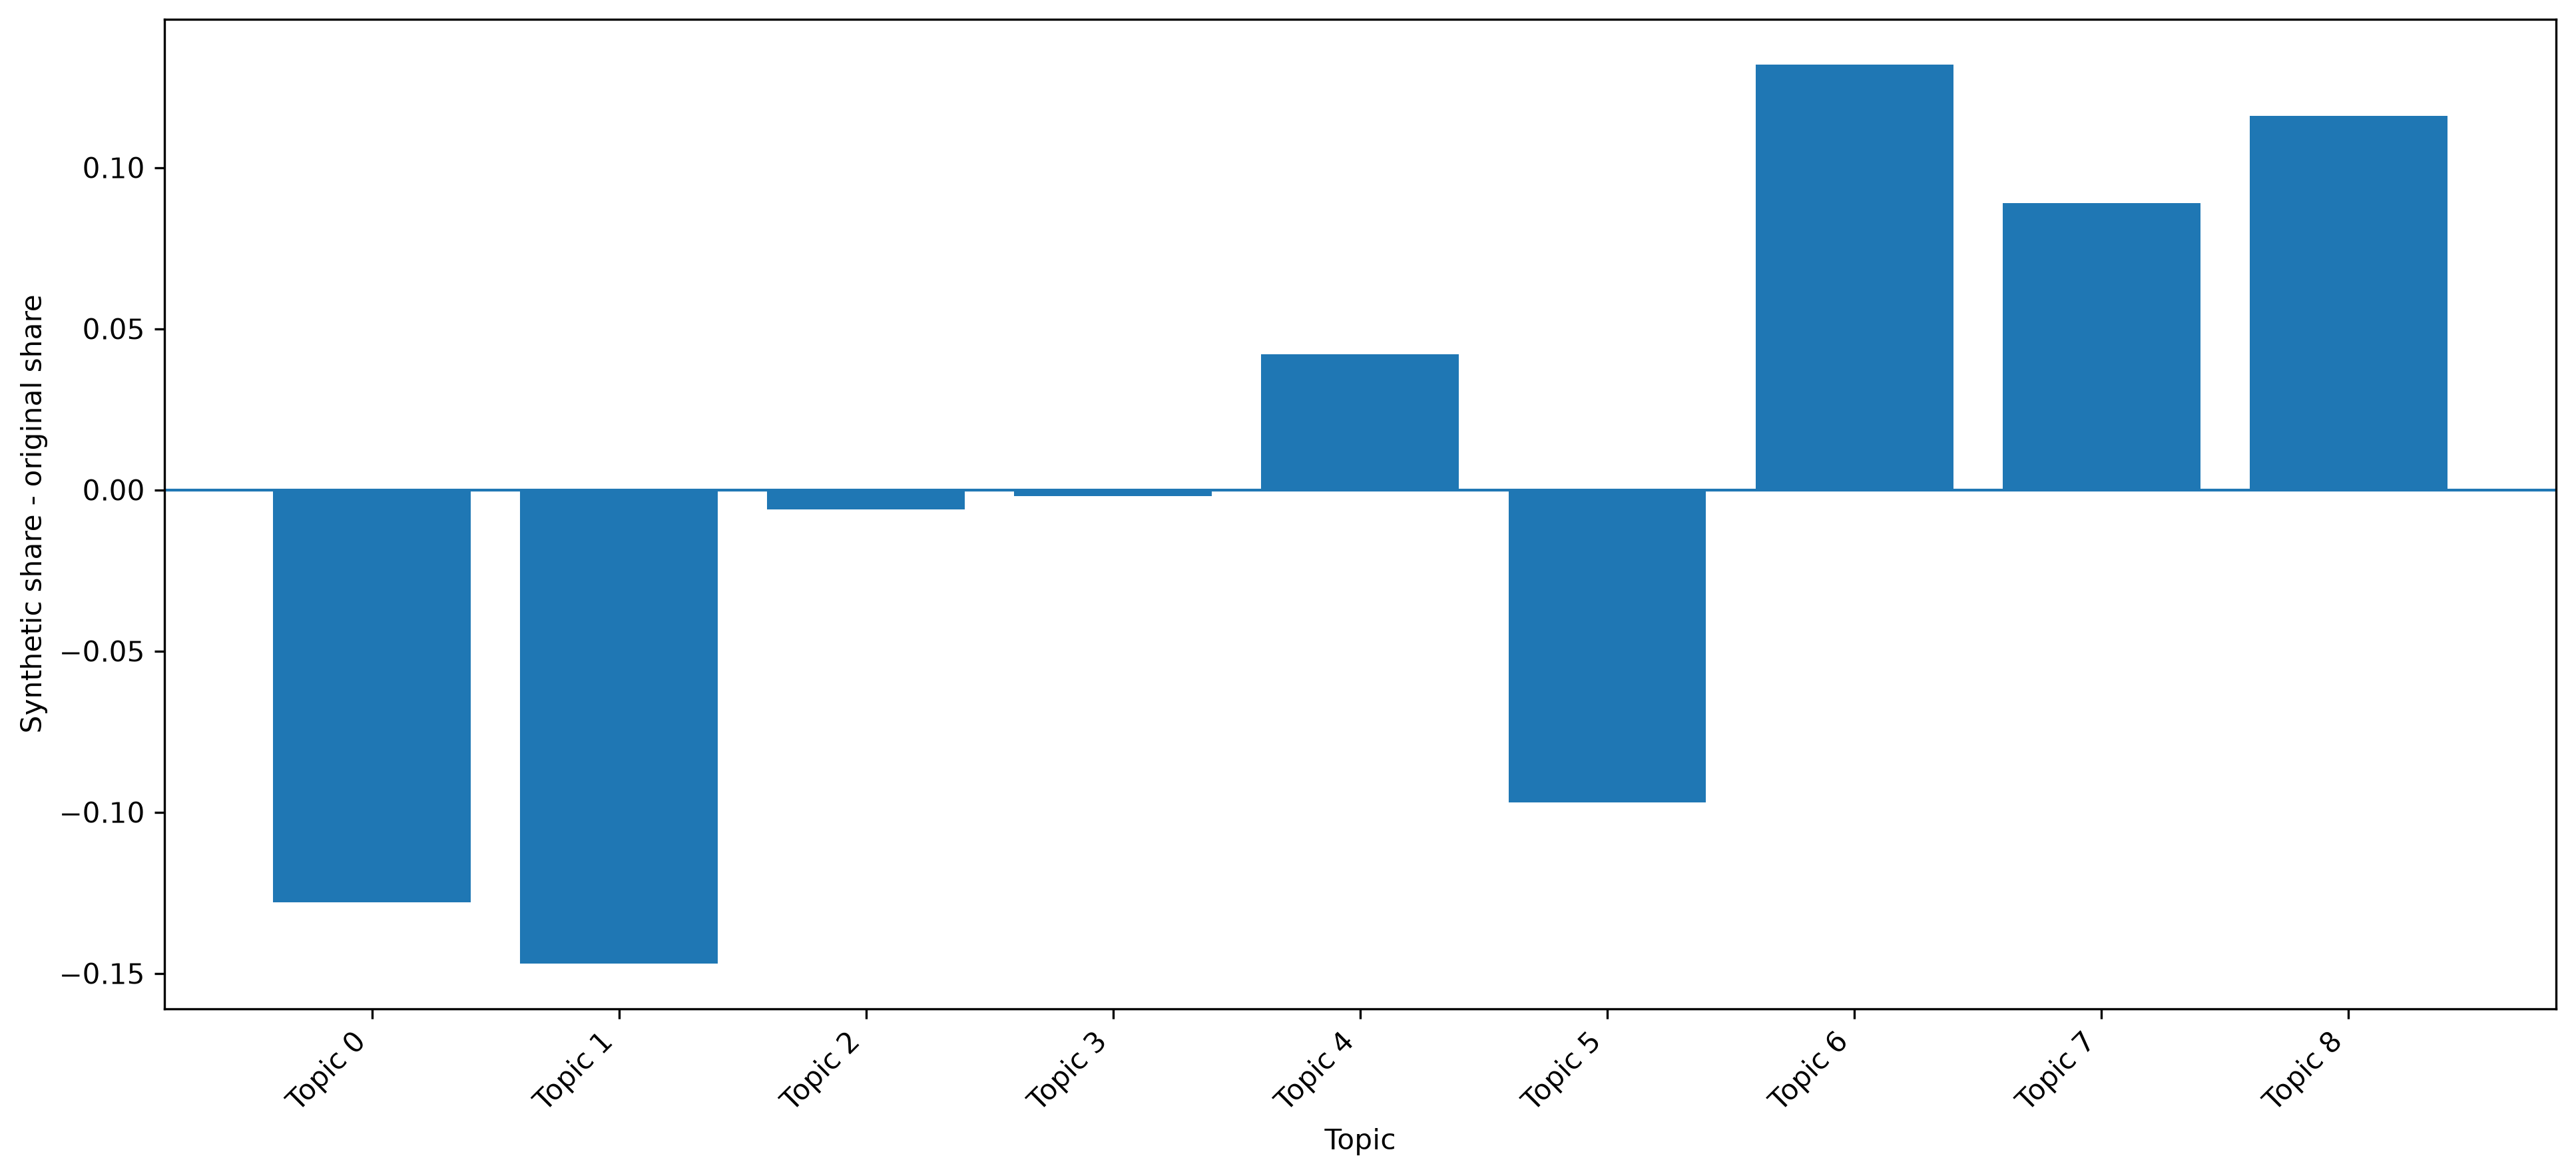
\includegraphics[scale=.24]{images/bert_sentiment_synthetic_share_difference.png}

    \caption{Sentiment BERTopic synthetic robustness results. Left: original versus synthetic sentiment topic distribution under the fitted BERTopic model. Right: difference between synthetic and original sentiment topic shares under the fitted BERTopic model.}
    \label{fig:bertopic-sentiment-synthetic-combined}
\end{figure}

The same pattern is clearer when the difference between synthetic and original topic
shares is plotted directly. Figure~\ref{fig:bertopic-sentiment-synthetic-combined}
(right) shows which topics are over-represented or under-represented by the synthetic
subset. Positive values indicate topics that receive proportionally more synthetic
chunks than original chunks, while negative values indicate topics that are weakly
represented or missing in the synthetic subset. This signed difference makes the
robustness finding more explicit: the synthetic data does not simply add more
examples, but changes the relative emphasis of the sentiment topic space. This
reinforces the need to treat synthetic chunks as a diagnostic distribution rather
than as additional evidence for the real sentiment corpus.


BERTopic improved over LDA by introducing a clustering-based view of the corpora and
by separating several themes that LDA had grouped together. However, its outputs
still depend on clustering decisions, and the topic-number search balances several
competing signals. The sentiment robustness check also shows that the synthetic
subset can over-emphasise specific concern-oriented topics.

For the final reference pipeline, NMF is therefore introduced next as a
factorisation-based model with explicit topic--word and document--topic matrices.
These matrices are easier to inspect, aggregate and reuse in the later
policy--sentiment gap analysis, while BERTopic remains a useful semantic-clustering
baseline.


\section{NMF as the reference factorisation pipeline}

Non-negative Matrix Factorisation (NMF) was used as the final reference
topic-modelling pipeline for the policy and sentiment corpora. NMF factorises a
non-negative document--term matrix into two non-negative matrices: a document--topic
matrix and a topic--word matrix. This makes it useful for this project because the
resulting topic weights are explicit, inspectable and easier to aggregate across
countries, corpora and later policy--sentiment comparisons
\cite{lee1999learning,xu2003document}.

Unlike BERTopic, which treats topic modelling as clustering, NMF keeps the model close
to the TF--IDF representation of the cleaned chunks. It therefore provides a stable
factorisation-based reference after the LDA and BERTopic baselines. As before, the SLM
was used only after topic modelling to phrase topic titles from keywords and
representative documents; it was not used to create the topic assignments.

\begin{verbatim}
Cleaned chunks
  -> TF--IDF document-term matrix
  -> search candidate NMF topic numbers
  -> evaluate coherence, cosine silhouette, diversity and topic balance
  -> fit the selected global model
  -> extract topic-word and document-topic matrices
  -> extract topic keywords and representative documents
  -> use a small language model only for topic phrasing
\end{verbatim}

The number of topics was selected using the same model-selection logic as the previous
pipelines. NPMI coherence was used to measure whether the top words of each topic form
an interpretable semantic group \cite{roder2015exploring}. Cosine silhouette was used
to check whether documents assigned to the same dominant topic were closer to each
other than to documents assigned to other topics \cite{rousseeuw1987silhouettes}.
Topic diversity was retained to penalise repeated or overlapping topic-word lists
\cite{dieng2020topic}. Topic balance was used as an internal diagnostic to avoid
models dominated by one very large topic. The final choice therefore had to balance
interpretability, separation, diversity and usable topic size.

\subsection{Policy NMF outcome}

For the global policy corpus, the NMF search selected nine topics. The selected model
had NPMI coherence 0.0953, cosine silhouette 0.6685, a largest topic share of 0.147,
a smallest topic share of 0.048, balance 0.853 and diversity 0.917.
Figure~\ref{fig:nmf-policy-combined} shows the topic-number search on the left and
the country-level distribution on the right. The nine-topic model was retained because
it gave the strongest overall quality within the selected range while avoiding the
large dominant topic produced by smaller models.

\begin{figure}[h]
    \centering
    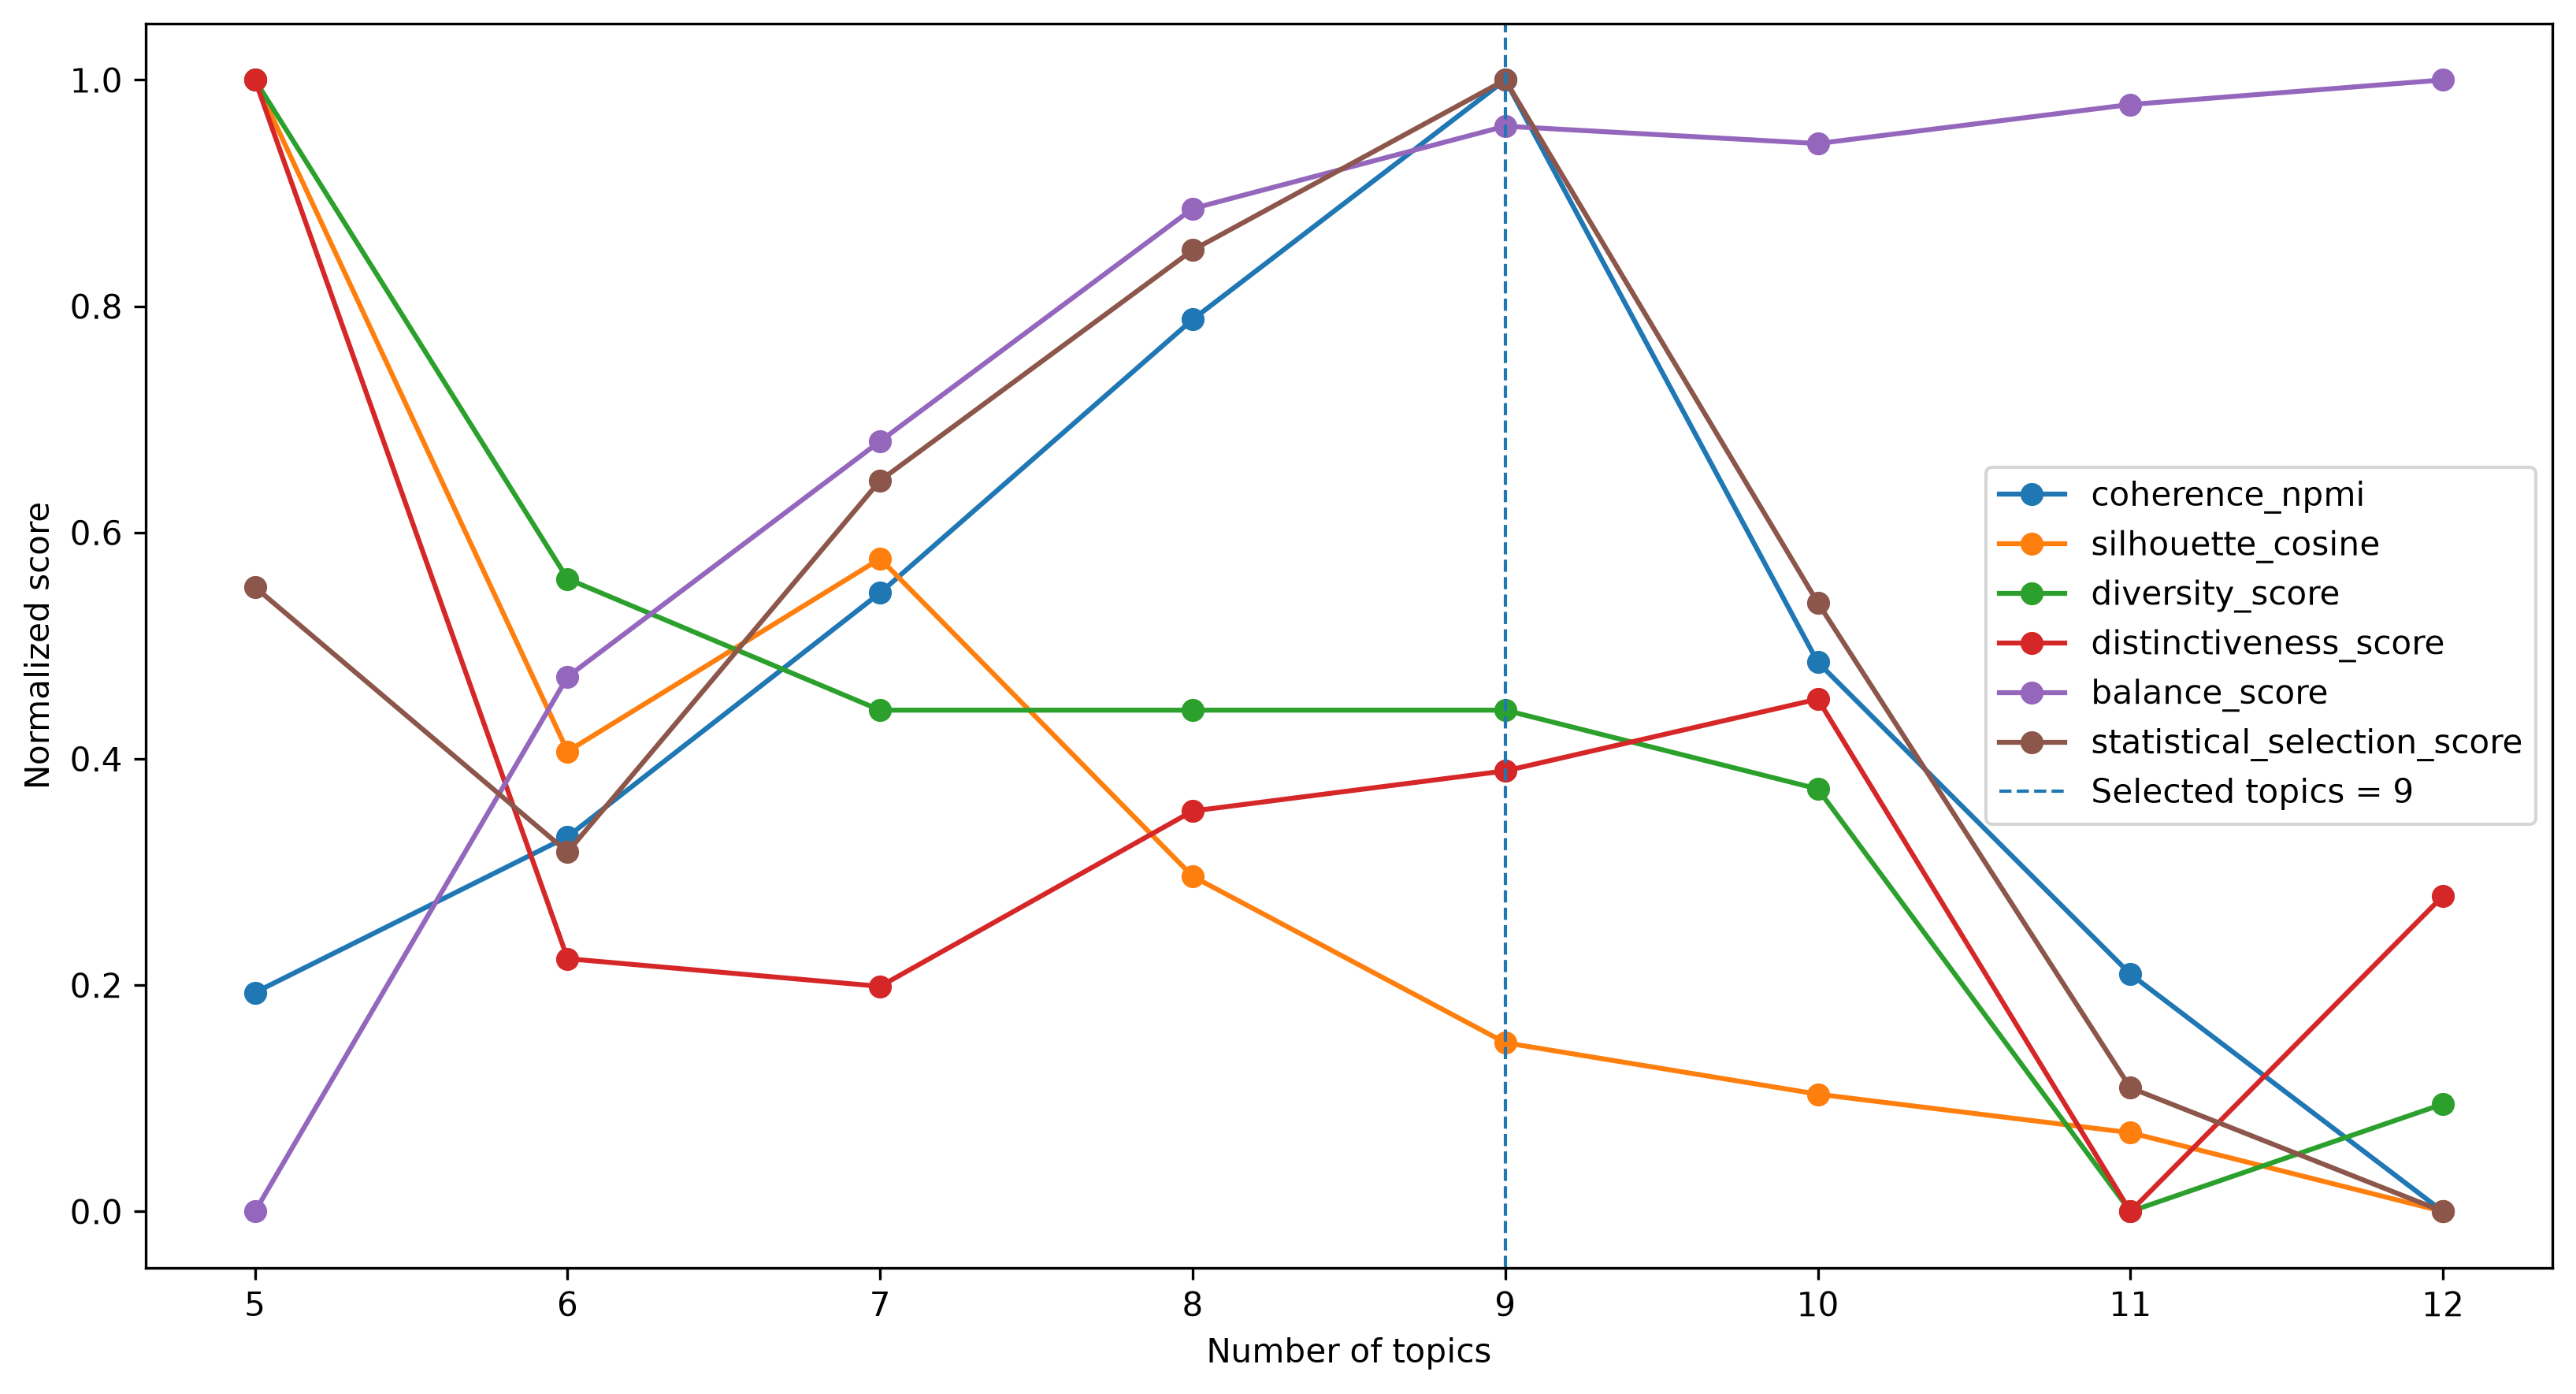
\includegraphics[width=0.42\linewidth]{images/policy_global_nmf_topic_selection_metrics.png}
    \hspace{0.04\linewidth}
    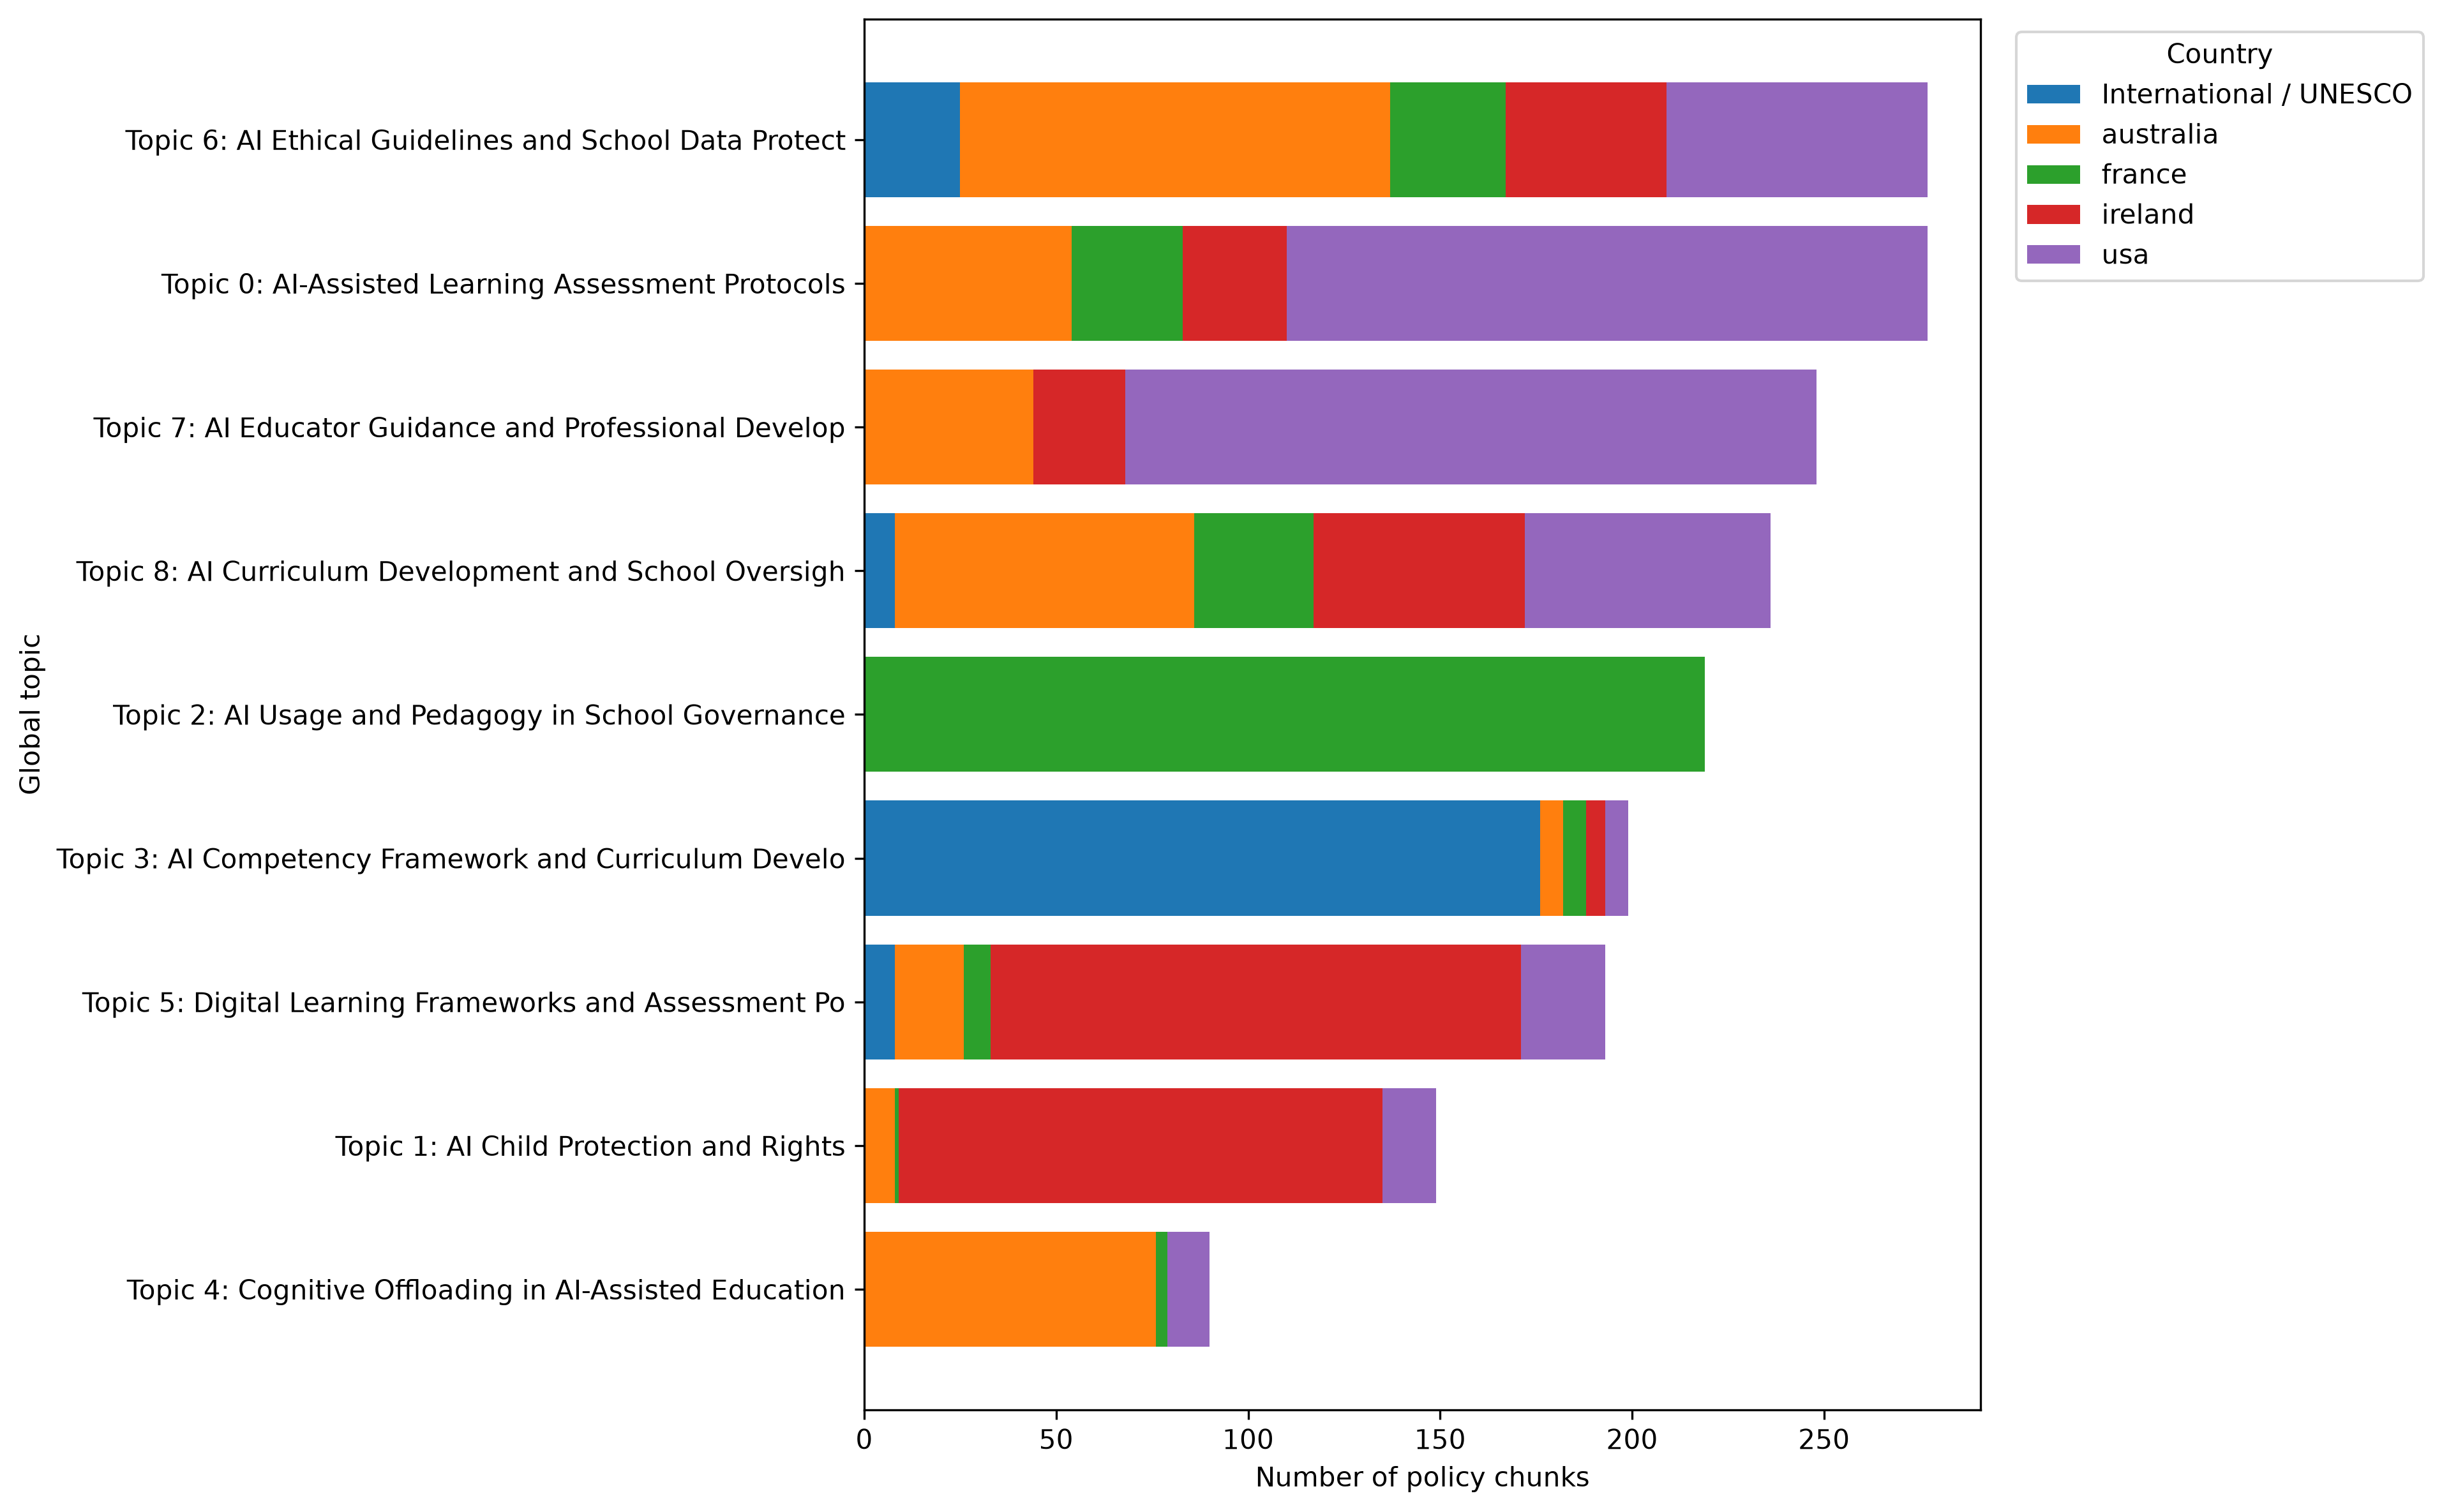
\includegraphics[width=0.42\linewidth]{images/policy_global_nmf_topic_distribution_by_country.png}

    \caption{Policy NMF results. Left: topic-number search using normalised coherence, cosine silhouette, diversity, balance and the combined selection score. Right: distribution of global policy NMF topics by country.}
    \label{fig:nmf-policy-combined}
\end{figure}

The global policy NMF topics are summarised in
Table~\ref{tab:nmf-policy-global-topics}. Compared with LDA, the model separates the
policy corpus into more specific education-governance themes. Compared with BERTopic,
it gives a more explicit topic--word and document--topic structure that can be reused
for aggregation and later comparison.

\begin{table}[h]
\centering
\small
\begin{tabular}{p{0.10\linewidth}p{0.16\linewidth}p{0.58\linewidth}}
\hline
Topic & Share & SLM topic phrase \\
\hline
0 & 0.147 & AI-assisted learning assessment protocols \\
1 & 0.079 & AI child protection and rights \\
2 & 0.116 & AI usage and pedagogy in school governance \\
3 & 0.105 & AI competency framework and curriculum development \\
4 & 0.048 & Cognitive offloading in AI-assisted education \\
5 & 0.102 & Digital learning frameworks and assessment policies \\
6 & 0.147 & AI ethical guidelines and school data protection \\
7 & 0.131 & AI educator guidance and professional development \\
8 & 0.125 & AI curriculum development and school oversight \\
\hline
\end{tabular}
\caption{Global policy NMF topics after SLM phrasing. The SLM is used only to phrase discovered topics, not to create the topic assignments.}
\label{tab:nmf-policy-global-topics}
\end{table}

The country-level distribution shown on the right of
Figure~\ref{fig:nmf-policy-combined} was used to inspect how the same global policy
topics appear across national policy sources. Country-specific NMF models were also
fitted as a secondary check. Australia selected three topics, Ireland selected four
topics, and France and the USA each selected seven topics. This confirms the pattern
already observed with BERTopic: the global AI-in-education vocabulary is shared across
the corpus, but its thematic granularity differs by country.

\subsection{Sentiment NMF outcome and synthetic robustness}

The sentiment NMF pipeline used the same factorisation logic, but synthetic data was
again kept analytically separate. The original sentiment chunks were used to fit the
empirical NMF model. Synthetic sentiment chunks were then projected into the learned
topic space in order to test whether the discovered sentiment structure was stable
under artificial perturbation. As in the LDA and BERTopic stages, synthetic data is
therefore treated as robustness evidence, not as final empirical evidence
\cite{halterman2025synthetic,chen2023empirical,chim2025evaluating}.

For the original sentiment corpus, the final selected NMF model used nine topics. The
selected model had NPMI coherence 0.0191, cosine silhouette 0.7417, a largest topic
share of 0.198, a smallest topic share of 0.064, balance 0.802 and diversity 0.917.
Figure~\ref{fig:nmf-sentiment-search} shows the topic-number search. Although smaller
models produced competitive raw scores, the nine-topic model gave a more granular
sentiment map while still satisfying the balance and minimum-share constraints.

\begin{figure}[h]
    \centering
    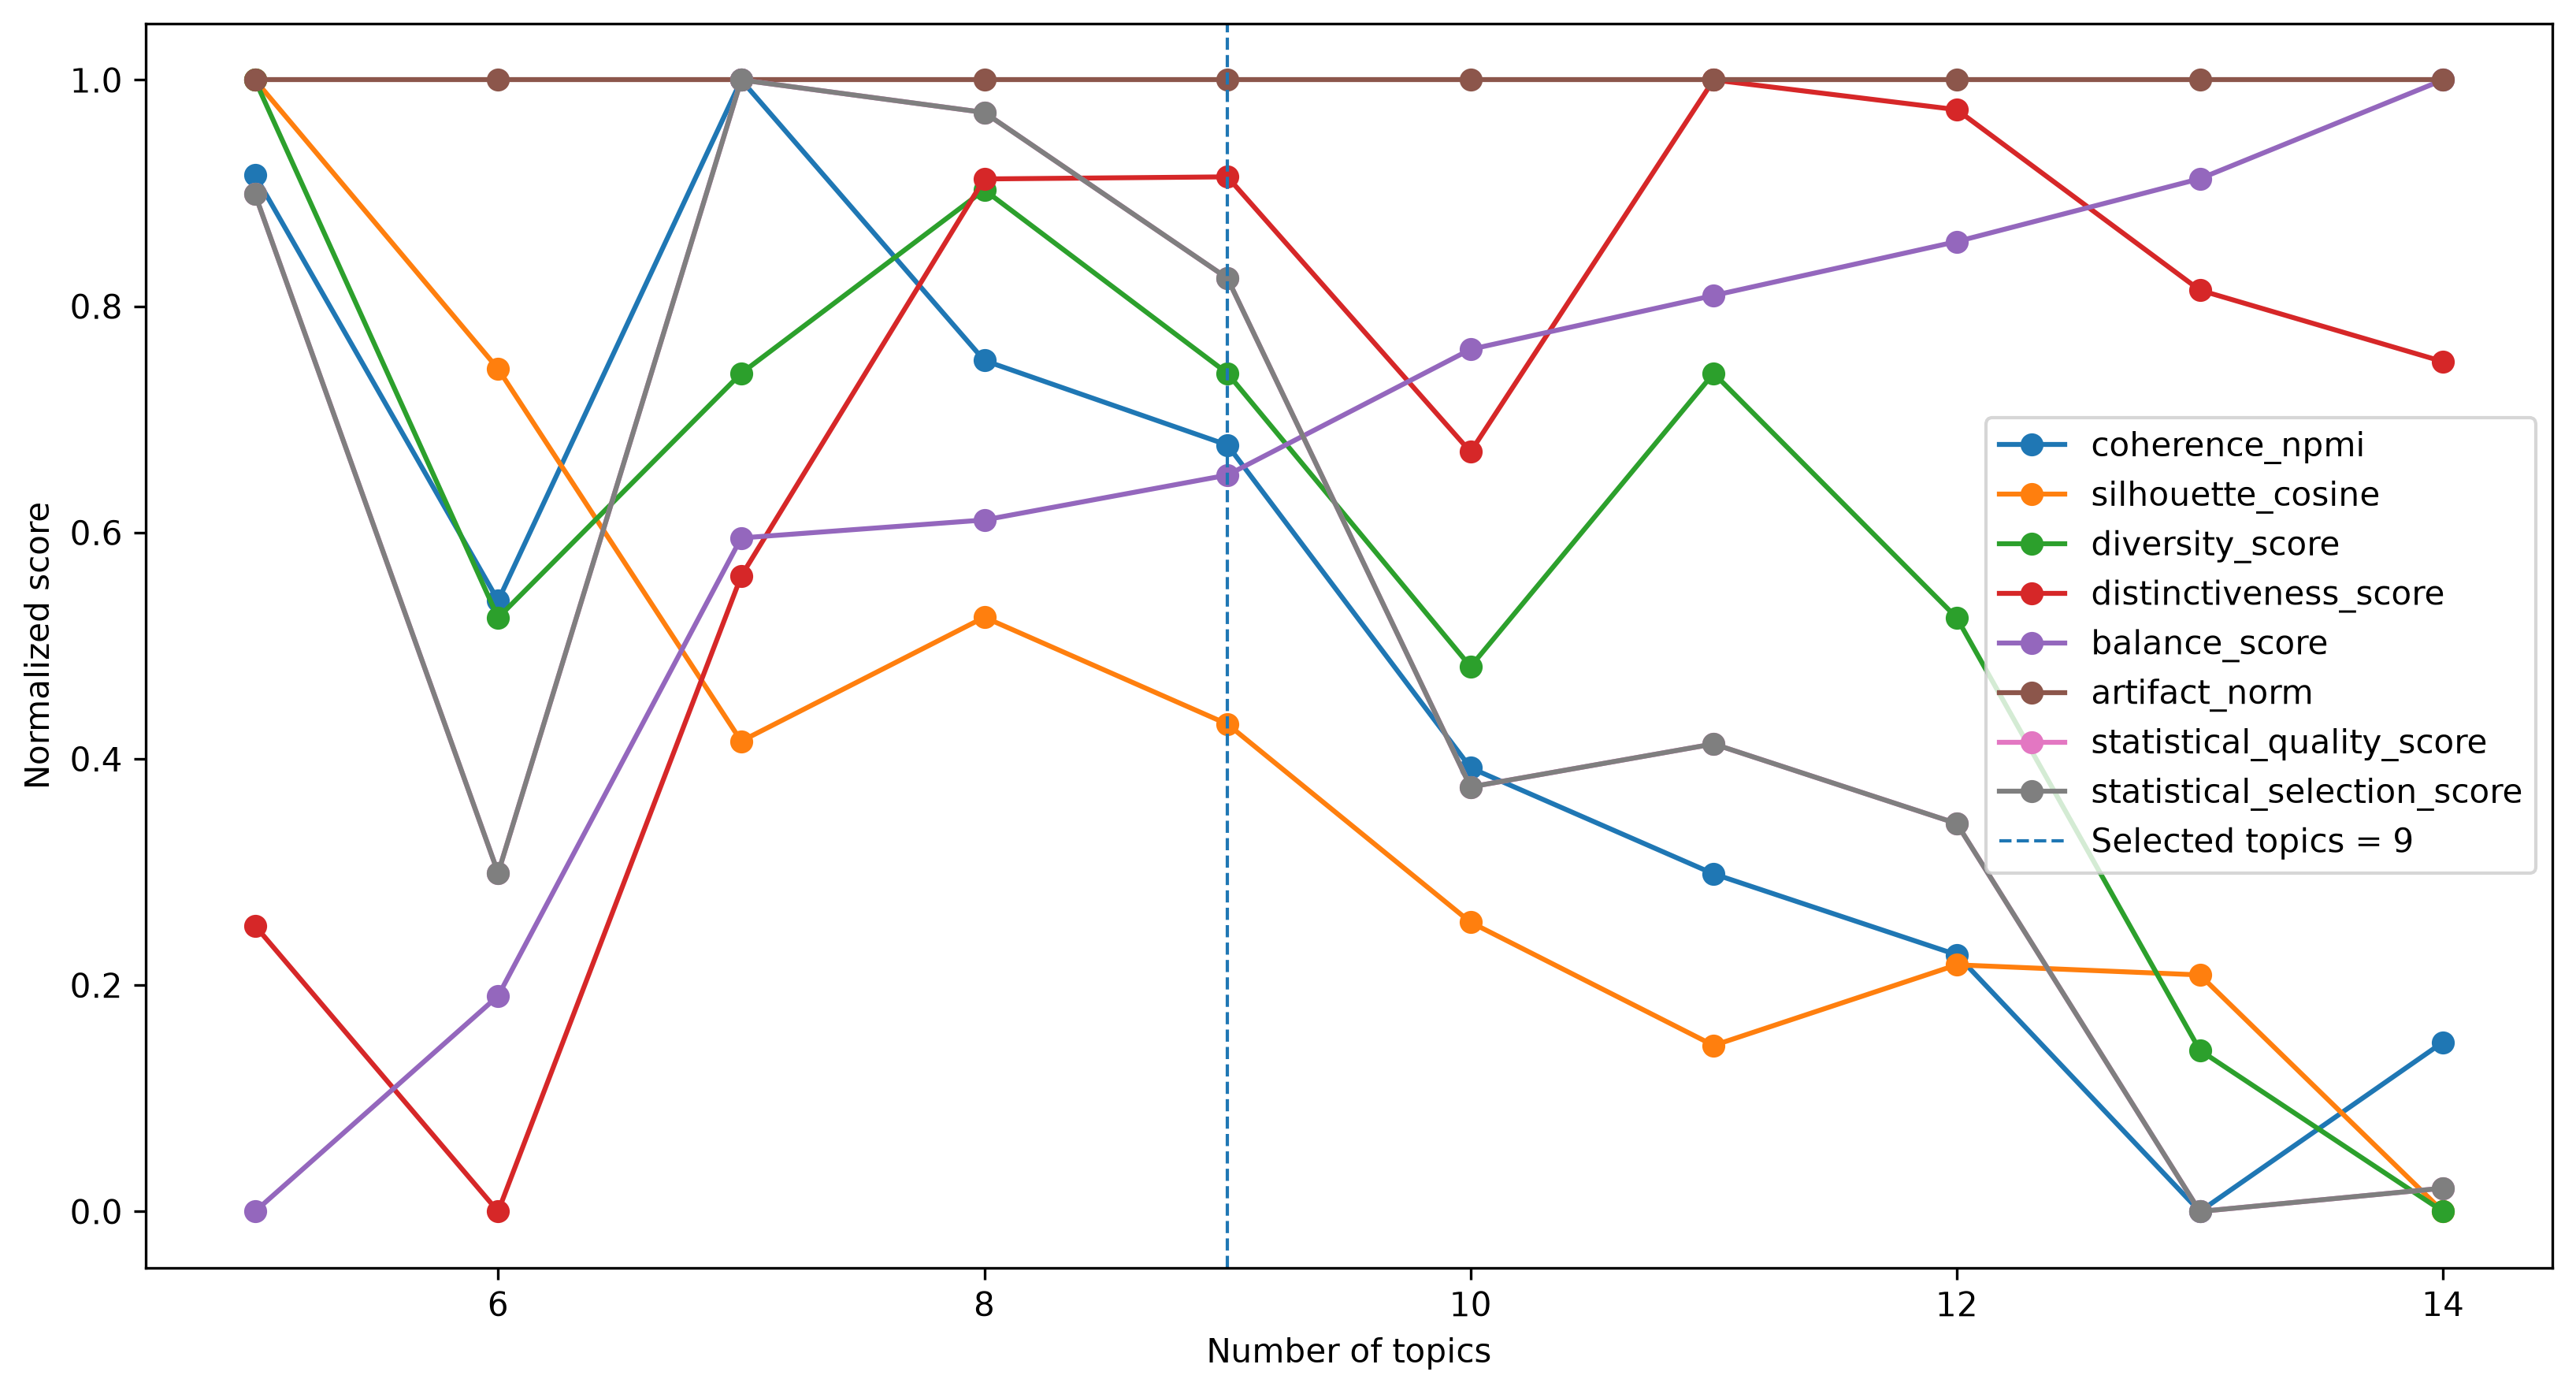
\includegraphics[scale=0.38]{images/sentiment_nmf_topic_selection_metrics.png}
    \caption{Sentiment NMF topic-number search using normalised coherence, cosine silhouette, diversity, balance and the combined selection score.}
    \label{fig:nmf-sentiment-search}
\end{figure}

The resulting sentiment topics mainly capture youth wellbeing, teacher adaptation,
GenAI assessment uncertainty, educator training, youth-work perspectives, teacher
experience, public fears and hopes, online learning clarity and digital technology
effects. The topic shares and SLM-generated phrases are summarised in
Table~\ref{tab:nmf-sentiment-topics}. This provides the most structured sentiment map
used in the topic-modelling comparison.

\begin{table}[h]
\centering
\small
\begin{tabular}{p{0.10\linewidth}p{0.16\linewidth}p{0.58\linewidth}}
\hline
Topic & Share & SLM topic phrase \\
\hline
0 & 0.081 & Young people's AI impact on education and well-being \\
1 & 0.158 & Student engagement and teacher adaptation to AI in classrooms \\
2 & 0.073 & GenAI detection and assessment confusion among learners and staff \\
3 & 0.198 & Educator training and ethical AI integration \\
4 & 0.121 & Youth workers' perspectives on AI integration \\
5 & 0.147 & Teachers' experience and knowledge in AI integration \\
6 & 0.086 & Public perception of AI in youth employment \\
7 & 0.073 & Online learning intention clarity and classroom relevance \\
8 & 0.064 & Impact of digital technologies on youth and education \\
\hline
\end{tabular}
\caption{Original sentiment NMF topics after SLM phrasing. The labels are generated after factorisation and are used for readability only.}
\label{tab:nmf-sentiment-topics}
\end{table}


\begin{figure}[h]
    \centering
    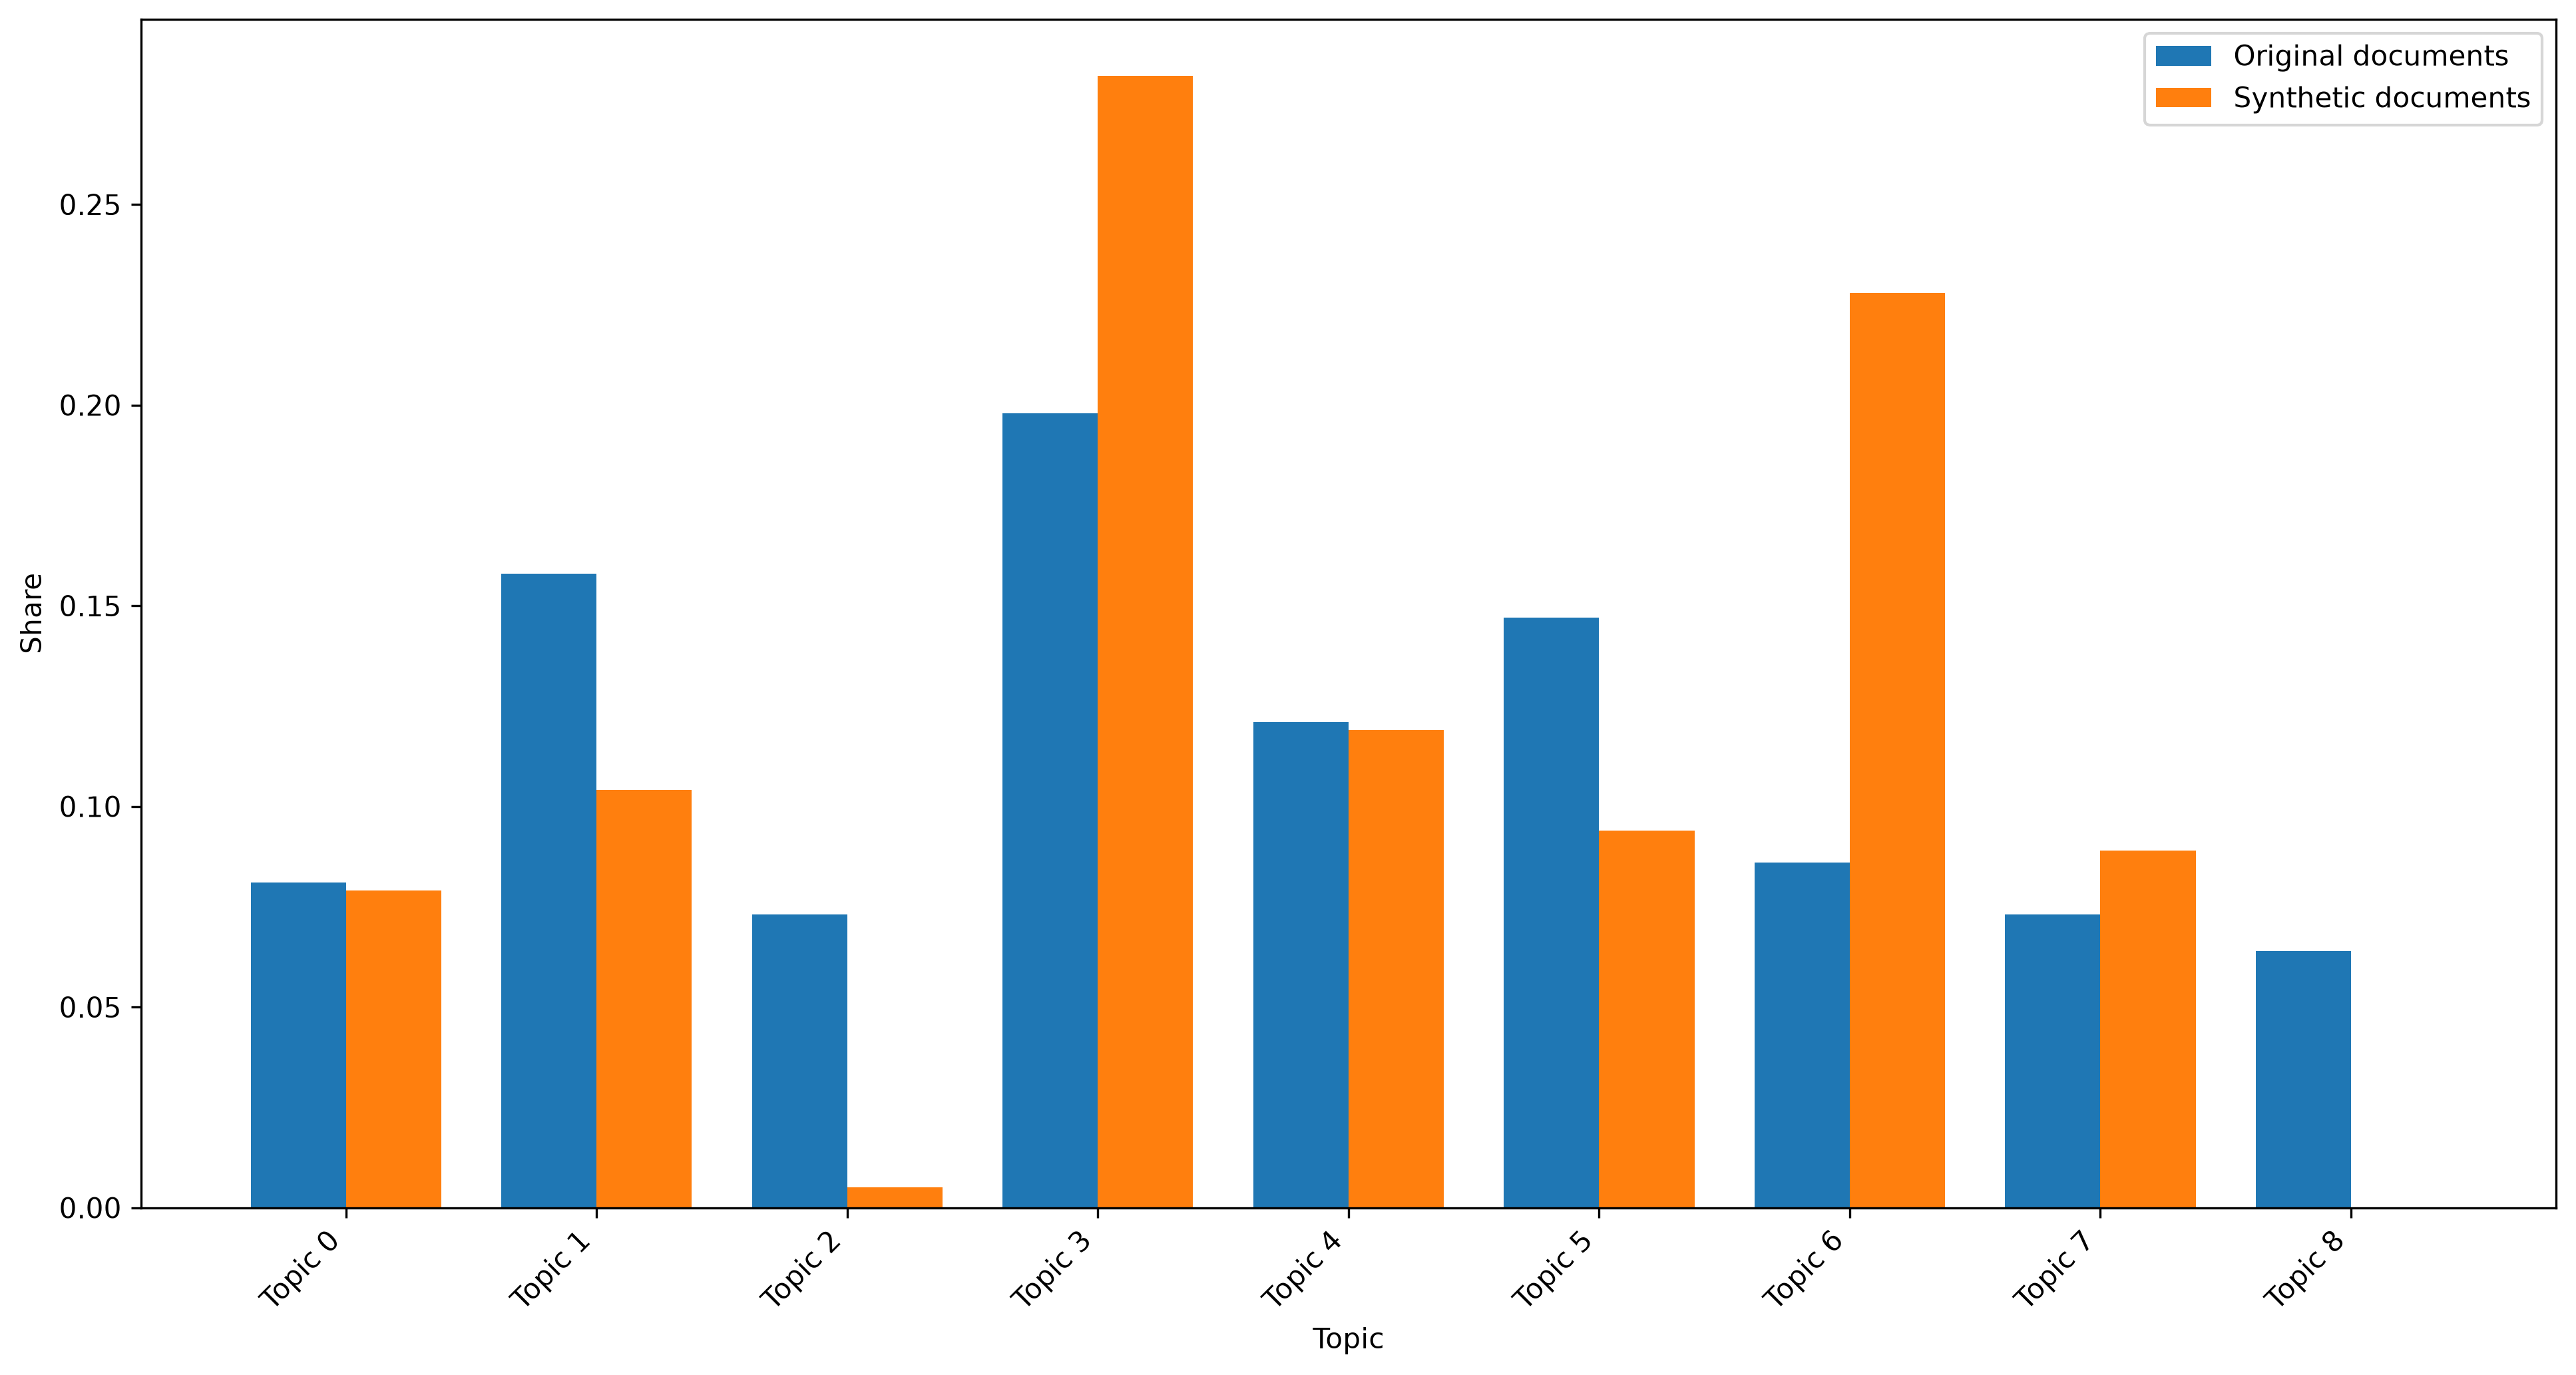
\includegraphics[width=0.42\linewidth]{images/sentiment_nmf_original_vs_synthetic_distribution.png}
    \hspace{0.04\linewidth}
    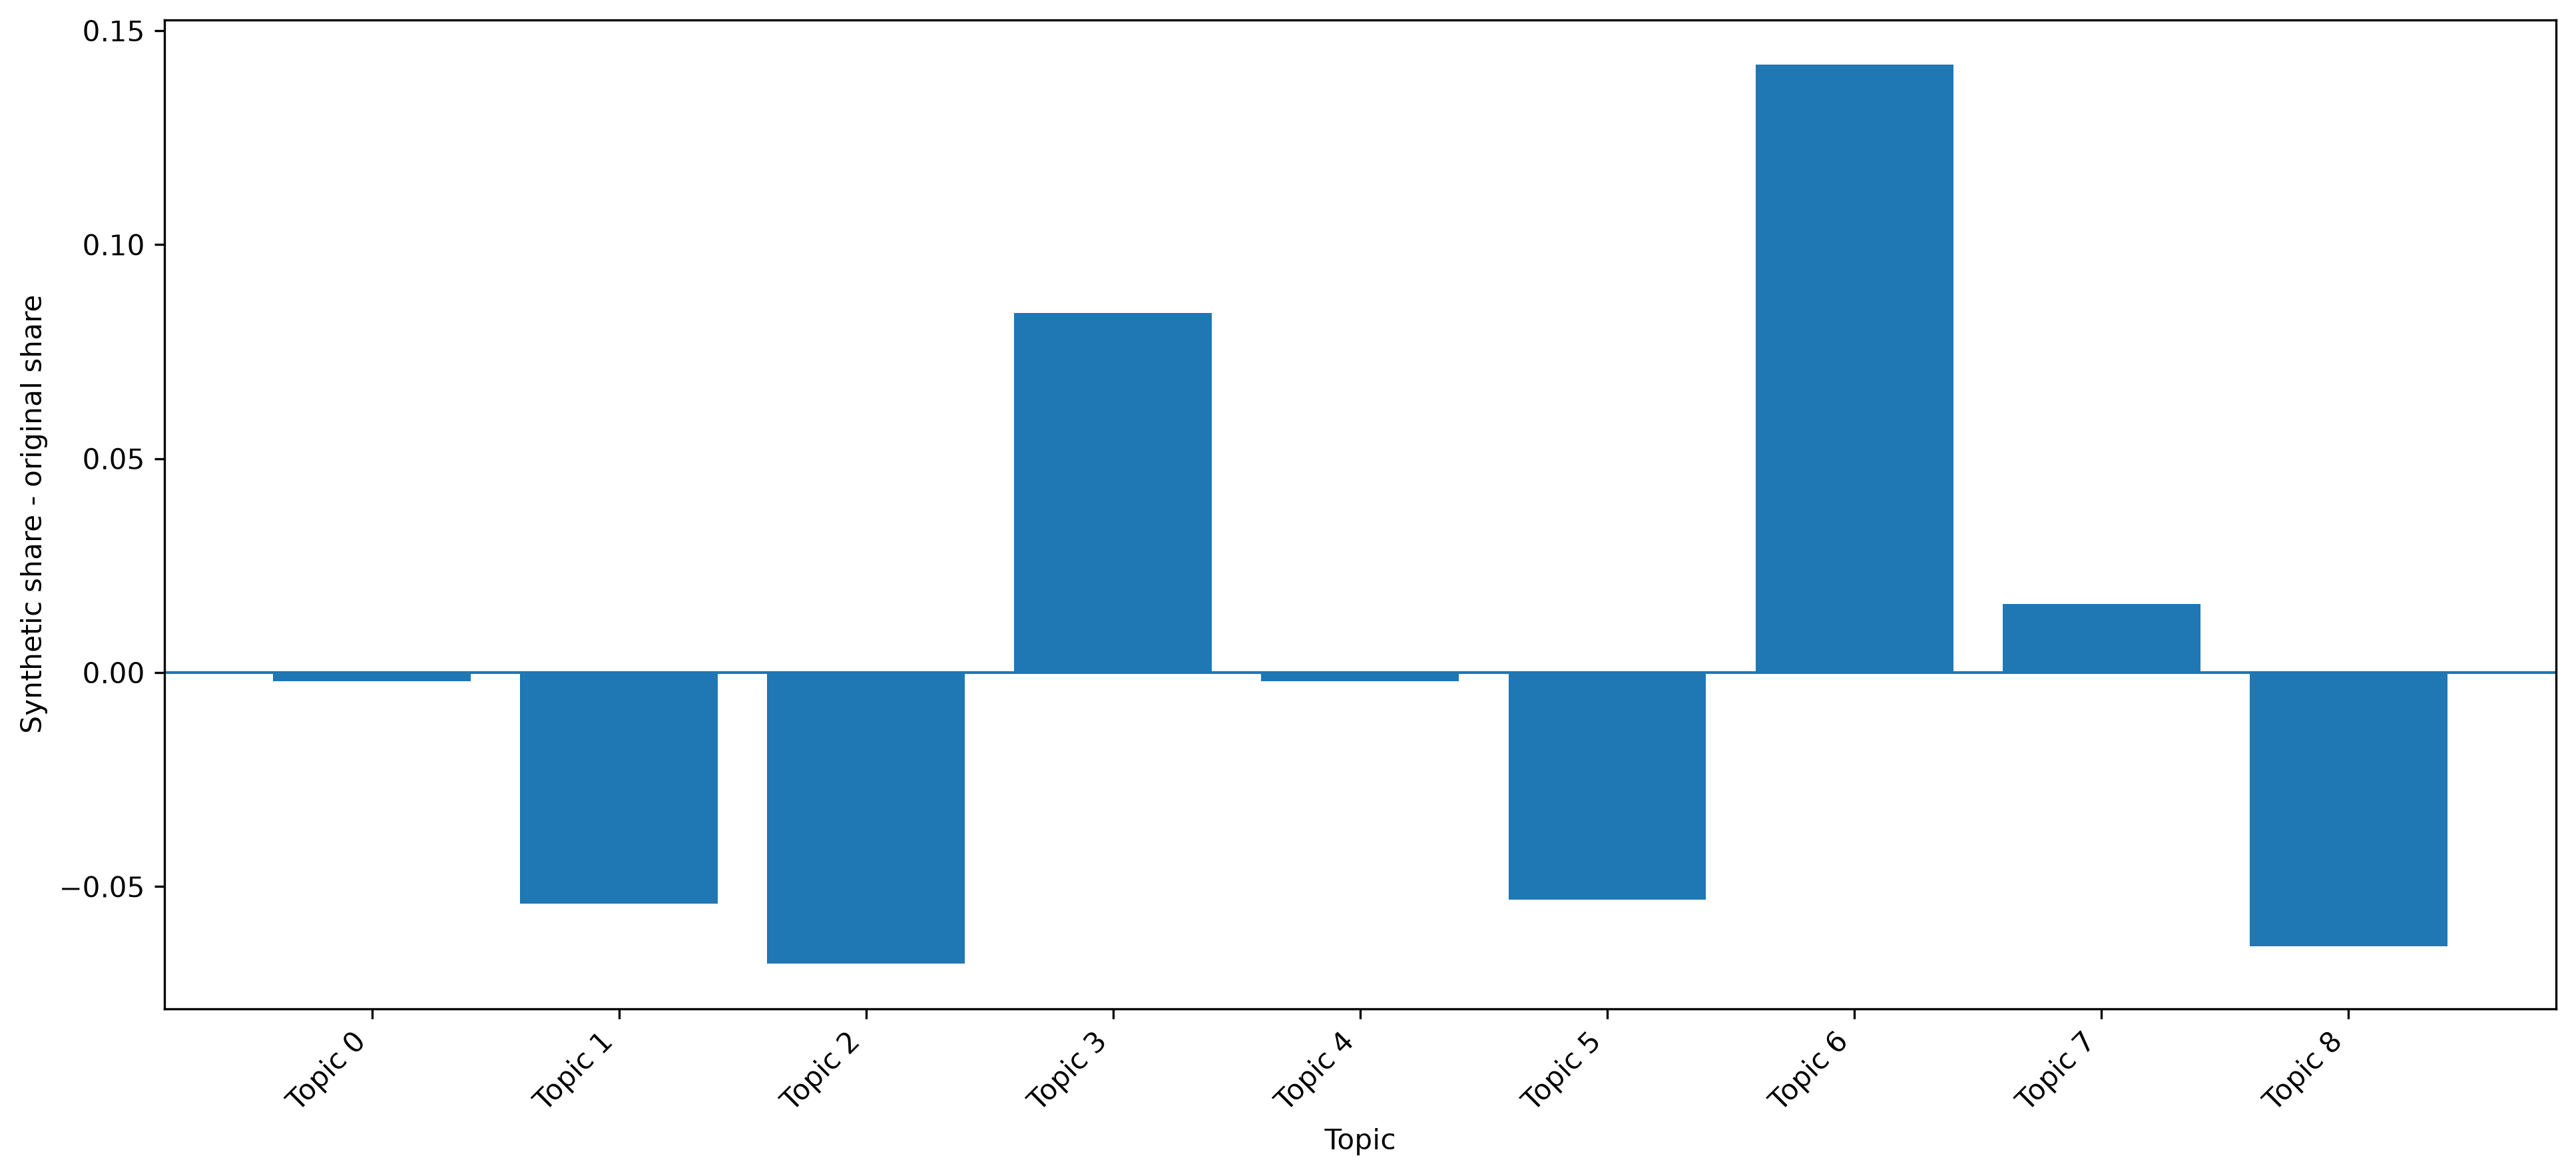
\includegraphics[width=0.42\linewidth]{images/sentiment_nmf_synthetic_share_difference.png}

    \caption{Sentiment NMF synthetic robustness results. Left: original versus synthetic sentiment topic distribution under the fitted NMF model. Right: difference between synthetic and original sentiment topic shares under the fitted NMF model.}
    \label{fig:nmf-sentiment-synthetic-combined}
\end{figure}

The synthetic robustness check showed that synthetic sentiment chunks did not
preserve the same topic proportions as the original sentiment corpus.
Figure~\ref{fig:nmf-sentiment-synthetic-combined} compares the original and synthetic
topic distributions on the left and shows the signed share difference on the right.
The largest synthetic over-representation appeared in topics linked to educator
training and public perception, while topics linked to GenAI assessment confusion,
teacher experience and digital technology effects were under-represented or missing
from the synthetic subset.


This confirms the same methodological rule established earlier: synthetic text is
useful for stress testing the topic model, but it changes the relative emphasis of
the sentiment space. It should therefore not be merged with the original sentiment
corpus to define the final empirical topic structure.


Across the three topic-modelling stages, LDA provided a transparent lexical baseline,
BERTopic tested a clustering-based semantic alternative, and NMF provided the final
factorisation-based reference model. NMF is retained as the main topic representation
for the later policy--sentiment gap analysis because it offers explicit topic--word
and document--topic matrices, stable topic shares and a clearer basis for aggregation
across corpora and countries.

\section{Causal NLP Application for Policy-Sentiment Gap Discovery}

The next step builds on the NMF representation to move from topic discovery to gap
analysis. Because NMF produces explicit document--topic weights, each policy and
sentiment chunk can be represented by comparable topic-share vectors. These vectors
can then be used in a causal NLP layer to examine where policy emphasis and public or
educational sentiment diverge, for example when a policy topic is strongly
represented in national documents but weakly reflected in sentiment data, or when
sentiment concerns appear without a corresponding policy focus. In this sense, NMF
provides the measurement layer, while causal NLP is introduced next to analyse
potential policy--practice gaps rather than to redefine the topics themselves.


\bibliographystyle{abbrv}
\bibliography{references}

\end{document}
